%% Journal version (Springer Nature template, sn-jnl.cls).  Build: pdflatex, bibtex, pdflatex x2.
%% Numbers come from generated files (experiments/make_*_assets.py); do not edit them by hand.
\documentclass[pdflatex,sn-mathphys-num]{sn-jnl}

\usepackage{graphicx}
\usepackage{multirow}
\usepackage{amsmath,amssymb,amsfonts}
\usepackage{amsthm}
\usepackage{mathrsfs}
\usepackage[title]{appendix}
\usepackage{xcolor}
\usepackage{textcomp}
\usepackage{manyfoot}
\usepackage{booktabs}
\usepackage{tikz}
\usetikzlibrary{arrows.meta,positioning}

\theoremstyle{thmstyleone}
\newtheorem{theorem}{Theorem}
\newtheorem{proposition}[theorem]{Proposition}
\newtheorem{lemma}[theorem]{Lemma}
\newtheorem{corollary}[theorem]{Corollary}
\theoremstyle{thmstylethree}
\newtheorem{definition}{Definition}
\newtheorem{remark}{Remark}

\newcommand{\Cl}{\mathcal C}
\newcommand{\Cay}{\mathrm{Cay}}
\newcommand{\ev}{\mathrm{ev}}
\newcommand{\RXX}{\mathrm{RXX}}\newcommand{\RX}{\mathrm{RX}}\newcommand{\RY}{\mathrm{RY}}\newcommand{\RZ}{\mathrm{RZ}}
\newcommand{\CZ}{\mathrm{CZ}}\newcommand{\SX}{\mathrm{SX}}
\newcommand{\Sp}{\mathrm{Sp}}
\newcommand{\op}[1]{\lVert#1\rVert}
\newcommand{\Dw}{\mathbb D[\omega]}
\newcommand{\Zw}{\mathbb Z[\omega]}
\newcommand{\qcr}{\texttt{qcr}}

\newcommand{\DiamIonThree}{17}
\newcommand{\DiamIonThreePlusOne}{18}
\newcommand{\MeanIonThree}{10.72}
\newcommand{\DiamIbmThree}{19}
\newcommand{\MeanIbmThree}{12.34}
\newcommand{\BFSMinutes}{25}
\newcommand{\OddRelIon}{11}
\newcommand{\OddRelIonMinusOne}{10}
\newcommand{\OddRelIonHalf}{6}
\newcommand{\OddRelIonHalfMinusOne}{5}
\newcommand{\OddRelIbm}{9}
\newcommand{\TwoQThreeDist}{13{,}824/373{,}248/5{,}971{,}968/38{,}486{,}016/42{,}052{,}608/5{,}971{,}968/27{,}648 for $0/\dots/6$ entangling gates}
\newcommand{\TwoQThreeMean}{3.51}
\newcommand{\TwoQThreeMax}{6}
\newcommand{\OptIon}{10.4}
\newcommand{\FaithIon}{47.1}
\newcommand{\EWeightIon}{28.3}
\newcommand{\EWsixteenIon}{10.4}
\newcommand{\FaithIonSec}{51}
\newcommand{\EWeightIonSec}{0.54}
\newcommand{\EWsixteenIonSec}{0.24}
\newcommand{\GapFactorIon}{4.5}
\newcommand{\SpeedupIon}{210}
\newcommand{\WStarIon}{12}
\newcommand{\OptIbm}{12.2}
\newcommand{\FaithIbm}{36.8}
\newcommand{\EWeightIbm}{51.1}
\newcommand{\EWsixteenIbm}{12.2}
\newcommand{\FaithIbmSec}{17}
\newcommand{\EWeightIbmSec}{0.22}
\newcommand{\EWsixteenIbmSec}{0.09}
\newcommand{\GapFactorIbm}{3.0}
\newcommand{\SpeedupIbm}{190}
\newcommand{\WStarIbm}{16}
\newcommand{\GridEightFive}{46.1}
\newcommand{\GridEightInf}{17.9}
\newcommand{\MeanIonTwoEven}{5.90}
\newcommand{\MeanIonTwoOdd}{5.88}
\newcommand{\BetaTwo}{0.937}
\newcommand{\LMixTwo}{133}
\newcommand{\MixLThree}{100}
\newcommand{\LBFourIon}{11.1}
\newcommand{\LBFourIbm}{12.9}
\newcommand{\LBThreeCheck}{7.9}
\newcommand{\CWFourIon}{56.7}
\newcommand{\CWFourIonTwoQ}{27.6}
\newcommand{\CWFourSec}{5.6}
\newcommand{\EWFourSec}{0.8}
\newcommand{\FaithFourSec}{65}
\newcommand{\EWFourIon}{110.3}
\newcommand{\EWFourIonTwoQ}{44.2}
\newcommand{\FaithFourIon}{78.8}
\newcommand{\FaithFourIonTwoQ}{33.3}
\newcommand{\QFourIon}{164.9}
\newcommand{\QFourIonTwoQ}{47.3}
\newcommand{\FourImprovementIon}{49\%}
\newcommand{\QThreeIon}{127.2}
\newcommand{\CWFourIbm}{59.1}
\newcommand{\CWFourIbmTwoQ}{27.1}
\newcommand{\EWFourIbm}{130.9}
\newcommand{\EWFourIbmTwoQ}{47.1}
\newcommand{\FaithFourIbm}{76.0}
\newcommand{\FaithFourIbmTwoQ}{32.4}
\newcommand{\QFourIbm}{140.9}
\newcommand{\QFourIbmTwoQ}{47.3}
\newcommand{\FourImprovementIbm}{45\%}
\newcommand{\QThreeIbm}{104.0}
\newcommand{\GapFindings}{\paragraph{Findings.} (1) On its own benchmark the original method finishes \GapFactorIon$\times$ (ion trap) and
\GapFactorIbm$\times$ (IBM-style) above the exact optimum. Our faithful port reproduces the paper's single-circuit number
(\FaithIon\ vs.\ 45 gates), so the gap is a property of the method, not of our implementation. (2) EW-$w$ reaches the
\emph{proven} optimum on all 20 circuits once $w\ge\WStarIon$ (ion trap) or $w\ge\WStarIbm$ (IBM-style), in a fraction of a second.
This is the cascade of Prop.~\ref{prop:cascade}: the transition is sharp, between $w=8$ and $w=12$ (ion trap) or $w=16$ (IBM-style). (3) The grid (Fig.~\ref{fig:grid})
shows that the \emph{database radius}, not the window or the search strategy, is the binding constraint. At $r=5$, enlarging the
window from 8 to 16 lowers the mean excess only from 46 to 43 gates. At $w=8$, raising $r$ from 5 to $\infty$ lowers it from 46 to 18,
and for $w\ge12$ with $r\ge8$ the excess is at most 2 gates (ion trap; IBM-style: from 72 to $\le$\,8). Theorem~\ref{thm:exact} predicts
both requirements: windows long enough \emph{and} a database deep enough. The original method is limited by the second.
}
\newcommand{\FourFindings}{\paragraph{Findings.} (1) \emph{Convexity matters more than anything else at $n\ge4$.} With the same exact 3-qubit
oracle, contiguous windows (EW-16) give \EWFourIon\ (ion trap) and \EWFourIbm\ (IBM-style) gates, no better than the
published method. With DAG-convex windows (CW-24) the same oracle gives \CWFourIon\ and \CWFourIbm\ gates, i.e.\
\FourImprovementIon\ and \FourImprovementIbm\ fewer than the published results, in about \CWFourSec\,s per circuit. (2)
Two-qubit counts drop from 43 (published) to \CWFourIonTwoQ\ RXX and \CWFourIbmTwoQ\ CZ, on par with BQSKit L4 for the ion trap (28) and
below it for the IBM-style set (37), although CW optimises total length, not two-qubit count. (3) The certified lower bounds
(\LBFourIon, \LBFourIbm) leave a gap of at most a factor $\approx5$. Closing it, either by tightening the bound (deeper spheres,
meet-in-the-middle) or by better upper bounds (4-qubit oracles via symmetry reduction), is an open problem that our framework
makes precise.
}

% generated by experiments/make_general_assets.py -- do not edit
\newcommand{\HwCircuits}{60}
\newcommand{\HwCompared}{58}
\newcommand{\HeronFromLThreeBetter}{9}
\newcommand{\HeronFromLThreeEqual}{49}
\newcommand{\HeronFromLThreeWorse}{0}
\newcommand{\HeronFromLThreeTotalUp}{1}
\newcommand{\HeronFromLThreeSuccDown}{0}
\newcommand{\HeronEspLOneOverLThree}{1.11}
\newcommand{\HeronEspOursOverLOne}{1.09}
\newcommand{\HeronLThreeRz}{5297}
\newcommand{\HeronLThreePulse}{7218}
\newcommand{\HeronLThreeTwoq}{2889}
\newcommand{\HeronFromLThreeRz}{4436}
\newcommand{\HeronFromLThreePulse}{6139}
\newcommand{\HeronFromLThreeTwoq}{2830}
\newcommand{\HeronMaxQubits}{12}
\newcommand{\HeronMaxInput}{1008}
\newcommand{\HeronRuns}{360}
\newcommand{\HeronUnverified}{5}
\newcommand{\HeronMaxExactErr}{1.9\cdot10^{-11}}
\newcommand{\HeronMaxStateErr}{2\cdot10^{-12}}
\newcommand{\HeronMaxApproxErr}{6.4\cdot10^{-4}}
\newcommand{\HeronApproxWithinBound}{59}
\newcommand{\HeronAllLegal}{60}
\newcommand{\HeronStateEmpty}{5}
\newcommand{\HeronPhaseGadgetGates}{240}
\newcommand{\HeronMedianSec}{10.4}
\newcommand{\HeronMaxSec}{180}
\newcommand{\HeronTvdCircuits}{49}
\newcommand{\HeronTvdLThree}{0.137}
\newcommand{\HeronTvdLOne}{0.115}
\newcommand{\HeronTvdCount}{0.096}
\newcommand{\HeronTvdWTwo}{0.088}
\newcommand{\HeronTvdCal}{0.088}
\newcommand{\HeronCalBeatsLThree}{39}
\newcommand{\HeronCalBeatsCount}{41}
\newcommand{\IonFromLThreeBetter}{1}
\newcommand{\IonFromLThreeEqual}{57}
\newcommand{\IonFromLThreeWorse}{0}
\newcommand{\IonFromLThreeTotalUp}{28}
\newcommand{\IonFromLThreeSuccDown}{0}
\newcommand{\IonEspLOneOverLThree}{0.99}
\newcommand{\IonEspOursOverLOne}{1.02}
\newcommand{\IonLThreeRz}{2223}
\newcommand{\IonLThreePulse}{3824}
\newcommand{\IonLThreeTwoq}{1378}
\newcommand{\IonFromLThreeRz}{3622}
\newcommand{\IonFromLThreePulse}{2422}
\newcommand{\IonFromLThreeTwoq}{1376}
\newcommand{\IonMaxQubits}{12}
\newcommand{\IonMaxInput}{1008}
\newcommand{\IonRuns}{360}
\newcommand{\IonUnverified}{0}
\newcommand{\IonMaxExactErr}{8.2\cdot10^{-11}}
\newcommand{\IonMaxStateErr}{6\cdot10^{-12}}
\newcommand{\IonMaxApproxErr}{1.4\cdot10^{-4}}
\newcommand{\IonApproxWithinBound}{60}
\newcommand{\IonAllLegal}{60}
\newcommand{\IonStateEmpty}{7}
\newcommand{\IonPhaseGadgetGates}{52}
\newcommand{\IonMedianSec}{3.0}
\newcommand{\IonMaxSec}{96}
\newcommand{\IonTvdCircuits}{49}
\newcommand{\IonTvdLThree}{0.0091}
\newcommand{\IonTvdLOne}{0.0157}
\newcommand{\IonTvdCount}{0.0092}
\newcommand{\IonTvdWTwo}{0.0084}
\newcommand{\IonTvdCal}{0.0084}
\newcommand{\IonCalBeatsLThree}{29}
\newcommand{\IonCalBeatsCount}{26}
\newcommand{\PfOneLThreeTwoq}{0}
\newcommand{\PfOneOursTwoq}{139}
\newcommand{\PfOneLOneTwoq}{153}
\newcommand{\PfTwoLThreeTwoq}{0}
\newcommand{\PfTwoOursTwoq}{298}
\newcommand{\PfTwoLOneTwoq}{300}
\newcommand{\PaperBenchN}{250}
\newcommand{\PaperBenchOk}{250}
\newcommand{\TThreeGen}{10.8}
\newcommand{\TThreeGenSec}{2.6}
\newcommand{\TThreeN}{20}
\newcommand{\TThreePaper}{47.1}
\newcommand{\TThreePaperN}{20}
\newcommand{\TThreeGenOverPaper}{0.25}
\newcommand{\TThreeLThree}{127.2}
\newcommand{\TThreeCliff}{--}
\newcommand{\TThreeOpt}{10.4}
\newcommand{\TThreeAtOpt}{17}
\newcommand{\TFourGen}{12.5}
\newcommand{\TFourGenSec}{2.8}
\newcommand{\TFourN}{20}
\newcommand{\TFourPaper}{36.8}
\newcommand{\TFourPaperN}{20}
\newcommand{\TFourGenOverPaper}{0.42}
\newcommand{\TFourLThree}{104.0}
\newcommand{\TFourCliff}{--}
\newcommand{\TFourOpt}{12.2}
\newcommand{\TFourAtOpt}{18}
\newcommand{\NjpIonGen}{46.1}
\newcommand{\NjpIonGenSec}{7.7}
\newcommand{\NjpIonN}{100}
\newcommand{\NjpIonPaper}{78.8}
\newcommand{\NjpIonPaperN}{30}
\newcommand{\NjpIonGenOverPaper}{0.57}
\newcommand{\NjpIonLThree}{164.9}
\newcommand{\NjpIonCliff}{45.6}
\newcommand{\NjpIonOpt}{--}
\newcommand{\NjpIbmGen}{51.4}
\newcommand{\NjpIbmGenSec}{8.5}
\newcommand{\NjpIbmN}{100}
\newcommand{\NjpIbmPaper}{76.0}
\newcommand{\NjpIbmPaperN}{30}
\newcommand{\NjpIbmGenOverPaper}{0.70}
\newcommand{\NjpIbmLThree}{140.9}
\newcommand{\NjpIbmCliff}{49.3}
\newcommand{\NjpIbmOpt}{--}
\newcommand{\TFiveGen}{327.7}
\newcommand{\TFiveGenSec}{8.9}
\newcommand{\TFiveN}{10}
\newcommand{\TFivePaper}{335.9}
\newcommand{\TFivePaperN}{10}
\newcommand{\TFiveGenOverPaper}{0.98}
\newcommand{\TFiveLThree}{332.1}
\newcommand{\TFiveCliff}{324.6}
\newcommand{\TFiveOpt}{--}

% generated by experiments/make_general_assets.py -- do not edit
\newcommand{\HwRows}{%
TKET (FullPeepholeOptimise on L1) & \(\times\)1.02 & \(\times\)1.71 & \(\times\)1.16 && \(\times\)1.27 & \(\times\)1.79 & \(\times\)0.992\\
\midrule
ours, exact, from L1 & \(\times\)1.00 & \(\times\)0.84 & \(\times\)1.21 && \(\times\)0.95 & \(\times\)0.76 & \(\times\)1.002\\
ours, exact, from L3 & \(\times\)0.98 & \(\times\)0.87 & \(\times\)1.03 && \(\times\)1.00 & \(\times\)1.00 & \(\times\)1.001\\
ours, approximate ($\varepsilon=10^{-3}$), from L1 & \(\times\)1.01 & \(\times\)0.84 & \(\times\)1.21 && \(\times\)0.95 & \(\times\)0.75 & \(\times\)1.002\\
ours, state/measurement-aware, from L1 & \(\times\)0.77 & \(\times\)0.61 & \(\times\)1.28 && \(\times\)0.62 & \(\times\)0.50 & \(\times\)1.010\\
}

% generated by experiments/make_new_assets.py -- do not edit
\newcommand{\CTRadius}{5}
\newcommand{\CTBallSize}{698{,}512}
\newcommand{\CTBallLevels}{1, 34, 569, 6{,}744, 67{,}664, 623{,}500}
\newcommand{\CTBallMinutes}{8}
\newcommand{\CTCertified}{9}
\newcommand{\CTRandN}{100}
\newcommand{\CTRandCert}{99}
\newcommand{\CTRandGenAtOpt}{99/99}
\newcommand{\CTRandOrigAtOpt}{81/99}
\newcommand{\CTPlantN}{41}
\newcommand{\CTPlantGenAtOpt}{41}
\newcommand{\CTPlantOrigAtOpt}{40}
\newcommand{\CTPlantInputMean}{90.3}
\newcommand{\CTPlantOptMean}{6.1}
\newcommand{\CTPlantGenMean}{6.1}
\newcommand{\CTPlantOrigMean}{6.1}
\newcommand{\CTPlantQiskitMean}{7.7}
\newcommand{\LayN}{8}
\newcommand{\LayEspLThree}{0.63}
\newcommand{\LayEspNAOurs}{1.01}
\newcommand{\LayEspRel}{1.14}
\newcommand{\LayEspJoint}{1.14}
\newcommand{\LayTwoqLThree}{493}
\newcommand{\LayTwoqNA}{493}
\newcommand{\LayTwoqNAOurs}{485}
\newcommand{\LayTwoqRel}{485}
\newcommand{\LayTwoqJoint}{471}
\newcommand{\LayTvdN}{5}
\newcommand{\LayTvdLThree}{0.569}
\newcommand{\LayTvdNA}{0.332}
\newcommand{\LayTvdNAOurs}{0.325}
\newcommand{\LayTvdRel}{0.225}
\newcommand{\LayTvdJoint}{0.222}
\newcommand{\LayJointBeatsNA}{5}
\newcommand{\LayJointNAShare}{50\%}
\newcommand{\LayMaxErr}{2.5e-12}

% generated by experiments/make_large_assets.py -- do not edit
\newcommand{\LargeRows}{%
Qiskit level 1 & \(\times\)1.22 & \(\times\)1.13 & \(\times\)0.24 && \(\times\)1.40 & \(\times\)1.13 & \(\times\)0.851\\
TKET (FullPeepholeOptimise on L1) & \(\times\)1.07 & \(\times\)1.96 & \(\times\)0.27 && \(\times\)1.39 & \(\times\)1.87 & \(\times\)0.828\\
\midrule
ours, exact, from L1 & \(\times\)1.05 & \(\times\)0.78 & \(\times\)0.43 && \(\times\)0.96 & \(\times\)0.68 & \(\times\)1.033\\
ours, exact, from L3 & \(\times\)0.98 & \(\times\)0.81 & \(\times\)1.12 && \(\times\)1.00 & \(\times\)1.00 & \(\times\)1.011\\
}
\newcommand{\RuntimeRows}{%
Qiskit level 1 & -- & -- && 0.11 & 0.04\\
Qiskit level 3 & 0.03 & 0.01 && 0.12 & 0.05\\
TKET & 0.30 & 0.86 && 8.2 & 9.6\\
BQSKit level 2 (8 workers) & 14.7 & 4.8 && 132 & 34.2\\
BQSKit level 3 (8 workers) & 53.6 & 11.2 && 842 & 138\\
\midrule
ours, exact, from L1 & 10.4 & 3.0 && 853 & 187\\
ours, exact, from L3 & 6.0 & 4.8 && 117 & 57.1\\
}
\newcommand{\LargeOutputs}{176}
\newcommand{\LargeCertOk}{171}
\newcommand{\LargeCertPending}{5}
\newcommand{\LargeCircuits}{45}
\newcommand{\LargeCertRechecked}{2}
\newcommand{\LargeCertFirstRejected}{7}
\newcommand{\LargeCertMaxSteps}{544{,}922}
\newcommand{\LargeCertMaxSec}{6.8}
\newcommand{\LargeCertMedSec}{0.13}
\newcommand{\LargeCertMaxErr}{10^{-7}}
\newcommand{\LargeEspMin}{10^{-3}}
\newcommand{\LargeHeronEspN}{13}
\newcommand{\LargeHeronN}{22}
\newcommand{\LargeHeronPfN}{19}
\newcommand{\LargeHeronPending}{2}
\newcommand{\LargeHeronMinQubits}{14}
\newcommand{\LargeHeronMaxQubits}{95}
\newcommand{\LargeHeronMaxInput}{5{,}425}
\newcommand{\LargeHeronFromLThreeBetter}{20}
\newcommand{\LargeHeronFromLThreeEqual}{2}
\newcommand{\LargeHeronFromLThreeWorse}{0}
\newcommand{\LargeHeronFromLThreeTotalUp}{0}
\newcommand{\LargeHeronFromLThreeSuccDown}{0}
\newcommand{\LargeHeronFromLThreeAllSaved}{19\%}
\newcommand{\LargeHeronFromLThreeTwoqSaved}{2.1\%}
\newcommand{\LargeHeronFromLThreeEsp}{1.12}
\newcommand{\LargeHeronFromLThreeEspMedAll}{1.14}
\newcommand{\LargeHeronLOneTwoqFewer}{6}
\newcommand{\LargeHeronLOneTwoqMore}{16}
\newcommand{\LargeHeronLOneAllFewer}{22}
\newcommand{\LargeHeronLegal}{all}
\newcommand{\LargeIonEspN}{25}
\newcommand{\LargeIonN}{25}
\newcommand{\LargeIonPfN}{19}
\newcommand{\LargeIonPending}{1}
\newcommand{\LargeIonMinQubits}{14}
\newcommand{\LargeIonMaxQubits}{95}
\newcommand{\LargeIonMaxInput}{5{,}425}
\newcommand{\LargeIonFromLThreeBetter}{1}
\newcommand{\LargeIonFromLThreeEqual}{24}
\newcommand{\LargeIonFromLThreeWorse}{0}
\newcommand{\LargeIonFromLThreeTotalUp}{12}
\newcommand{\LargeIonFromLThreeSuccDown}{0}
\newcommand{\LargeIonFromLThreeAllSaved}{0\%}
\newcommand{\LargeIonFromLThreeTwoqSaved}{0.0\%}
\newcommand{\LargeIonFromLThreeEsp}{1.01}
\newcommand{\LargeIonFromLThreeEspMedAll}{1.01}
\newcommand{\LargeIonLOneTwoqFewer}{11}
\newcommand{\LargeIonLOneTwoqMore}{0}
\newcommand{\LargeIonLOneAllFewer}{19}
\newcommand{\LargeIonLegal}{all}
\newcommand{\LargeHeronMaxSec}{6.4}
\newcommand{\LargeIonMaxSec}{2.4}


\raggedbottom

\begin{document}

\title[Exact, hardware-aware local rewriting of quantum circuits]{Exact, hardware-aware local rewriting of quantum
circuits, with certified ground truth}

\author*[1]{\fnm{Arnav} \sur{Kapoor}}\email{kapoorarnav43@gmail.com}
\affil*[1]{\orgname{Indian Institute of Science Education and Research Bhopal}, \orgaddress{\city{Bhopal},
\state{Madhya Pradesh}, \country{India}}}

\abstract{Local rewriting shortens a quantum circuit by repeatedly replacing a short sub-circuit with a cheaper
equivalent one taken from a precomputed database. We give this family of methods a precise foundation and test it
against exact ground truth. Every useful notion of ``equivalent sub-circuit'' (exact, up to global phase, on the
$|0\rangle$ input, before measurement, up to a chip symmetry, within $\varepsilon$) is the orbit relation of a group
action, so databases are keyed by canonical orbit representatives and soundness and error accumulation follow from two
short propositions. On this basis we build a gate-set-agnostic optimiser with exact, state-aware and approximate
semantics, calibrated costs and connectivity-aware windows, and extend it with layout-aware rewriting, which places the
optimised circuit on the cheapest region of the chip. For the discrete gate sets of a recent proposal every circuit is
Clifford. We enumerate all 92,897,280 three-qubit elements and prove when local optimality is global. Beyond Clifford, we
use exact arithmetic over $\mathbb Z[1/\sqrt2, e^{i\pi/4}]$ to certify optimal lengths of two-qubit Clifford+T
circuits and build long benchmark circuits with planted, certified optima. Against this ground truth the optimiser
reaches the proven optimum on \TThreeAtOpt/20 and \TFourAtOpt/20 three-qubit benchmark circuits, where the original method
is $4.5\times$ and $3.0\times$ above it, and on \CTPlantGenAtOpt/\CTPlantN\ planted Clifford+T circuits. On \HwCompared\
algorithm circuits compiled by Qiskit for IBM Heron it removes 13\% of the gates without adding a two-qubit gate, and
layout-aware rewriting raises the estimated success probability over Qiskit's noise-aware layout by
$\times$\LayEspJoint\ (geometric mean). The numerical resynthesis compiler BQSKit needs fewer two-qubit gates than our
optimiser on most of these circuits, at the price of approximate outputs, more single-qubit gates and longer run times.
The two combine. Run on BQSKit's output, our optimiser removes a further \HeronStackAllSaved\ of the gates on
Heron, never adds a two-qubit gate and never lowers the estimated success probability.
On \LargeHeronN\ arithmetic circuits of up to \LargeHeronMaxQubits\ qubits it removes \LargeHeronFromLThreeAllSaved\ of the gates
left by Qiskit's level~3 on Heron. Each of these outputs carries a replay certificate, a log of local steps that an
independent checker verifies a few qubits at a time. Every reported output is verified.}

\keywords{quantum circuit optimization, peephole optimization, Clifford group, Clifford+T, Cayley graph, exact
synthesis, qubit mapping, noise-aware compilation}

\maketitle

%=====================================================================
\section{Introduction}\label{sec:intro}

Compiling a quantum circuit into a device's native gates leaves redundancy, and on noisy hardware every gate costs
fidelity. A common figure of merit, the estimated success probability (ESP), is the product of the fidelities of all
gates and measurements~\cite{nishio2020}. Rosenhahn, Osborne and Hirche~\cite{rosenhahn2025} recently proposed a simple,
gate-set-agnostic remedy. A circuit is viewed as a word over the native alphabet. A window of $2$--$8$ letters is
sampled and replaced by a shorter equivalent word, found by random sampling (V1), by lookup in an exhaustively
enumerated database of short circuits (V2), or by a lookup gated by a random forest (V3). The method belongs to a long
line of database-driven, template and peephole optimisers~\cite{prasad2006,golubitsky2012,nam2018,iten2022,
bravyi2021templates,quartz,queso,quarl}.

Two questions decide whether such a method is worth using, and neither is answered in~\cite{rosenhahn2025}.
\emph{How far from optimal is it?} Results there are compared only with Qiskit~\cite{qiskit2024}, so it cannot be told
whether a 45-gate output for a 3-qubit circuit is good. We show that the optimum is about 10. \emph{Does it help on
circuits and hardware that matter?} The gate sets there are discrete $\pm\pi/2$ rotations with all-to-all
connectivity, the benchmarks are random words over these alphabets, and the objective is the total gate count.

This paper answers both questions with two strictly separated ingredients, a \emph{general optimiser} that uses no
structure of the gate set and \emph{exact ground truth} that does, used only for evaluation.

\paragraph{Contributions.}
\begin{enumerate}
\item \emph{A unifying model.} Equivalence notions are group actions and database keys are canonical orbit
  representatives (Table~\ref{tab:actions}). Soundness of state- and measurement-aware rewriting and an additive error
  bound for approximate rewriting follow (Propositions~\ref{prop:sound} and~\ref{prop:approx}).
\item \emph{A general optimiser} with exact global-phase handling, calibrated costs and connectivity-aware convex
  windows (Section~\ref{sec:engine}), and \emph{layout-aware rewriting}: noise-aware relocation of the optimised circuit
  and layout selection by post-optimisation cost (Section~\ref{sec:layout}).
\item \emph{Theory for discrete gate sets.} An exactness threshold for local rewriting, a parity theorem, mixing of
  random-circuit benchmarks, and counting lower bounds (Section~\ref{sec:theory}).
\item \emph{Certified ground truth.} Complete distance tables of the 3-qubit Clifford group under both alphabets
  of~\cite{rosenhahn2025}, and, beyond Clifford, exact two-qubit Clifford+T distances in the ring $\Dw$ together with
  long benchmark circuits whose optimum is planted and certified (Section~\ref{sec:exact}).
\item \emph{Experiments} on the original benchmarks, on certified Clifford+T benchmarks, and on \HwCompared\ algorithm
  circuits for IBM Heron and trapped-ion models and on arithmetic circuits of up to \LargeHeronMaxQubits\ qubits, against
  Qiskit, TKET~\cite{tket2021} and BQSKit~\cite{bqskit}, with every output verified, beyond the reach of statevector
  simulation by \emph{replay certificates} (Sections~\ref{sec:engine} and~\ref{sec:exp}).
\end{enumerate}
Section~\ref{sec:related} reviews related work, Section~\ref{sec:prelim} fixes notation, Section~\ref{sec:discussion}
discusses limitations, and the appendices summarise the reproduction of~\cite{rosenhahn2025}. The implementation,
\qcr, and every script and raw result are openly available (see Declarations).

%=====================================================================
\section{Related work}\label{sec:related}

\paragraph{Local and database-driven optimisation.} Peephole optimisation with databases of optimal small circuits goes
back to reversible logic~\cite{prasad2006,golubitsky2012}. For quantum circuits, rule-based optimisers with continuous
parameters~\cite{nam2018}, exact template matching~\cite{iten2022} and Clifford templates with symbolic Pauli
gates~\cite{bravyi2021templates} are standard. Superoptimisers enumerate small circuits, collect equivalent pairs and
use them as rewrite rules~\cite{quartz,queso}, and Quarl learns where to apply them~\cite{quarl}. The method
of~\cite{rosenhahn2025} is the database variant in its simplest form. Our optimiser keeps its simplicity but changes what
is stored (canonical orbit keys), where it is applied (DAG-convex windows on coupled qubits) and what it optimises
(calibrated cost). Resynthesis compilers take the opposite route. BQSKit~\cite{bqskit} partitions a circuit into blocks
of a few qubits and synthesises each block anew by numerical optimisation over parametrised circuit
templates~\cite{qsearch,leap}. It is not limited to stored rewrites, but its blocks are equal to their originals only up
to a numerical tolerance.

\paragraph{Optimal synthesis and exact ground truth.} Clifford circuits are described exactly by stabiliser
tableaux~\cite{aaronson2004}, have a complete set of relations~\cite{selinger2015}, and optimal circuits are known up to
six qubits~\cite{bravyi2022six}, and ZX-calculus simplification gives strong heuristics~\cite{duncan2020}. Clifford+T
unitaries are exactly those with entries in $\mathbb Z[1/\sqrt2, i]$~\cite{giles2013}. Single-qubit normal forms are
T-optimal~\cite{matsumoto2008,kmm2013}, rotations are approximated optimally~\cite{rossselinger2016}, and
meet-in-the-middle search gives depth- and T-count-optimal circuits for small
instances~\cite{amy2013mitm,gosset2014}. We use the same ingredients for a different purpose, namely certified optimal lengths
over a \emph{native hardware alphabet}, as a benchmark for heuristic optimisers. Benchmarks with known optimal solutions
have been advocated for qubit mapping~\cite{tan2021queko}, and our planted circuits play this role for gate-count
optimisation.

\paragraph{Layout and noise-aware compilation.} Qubit mapping and routing~\cite{li2019sabre} and noise-adaptive
mapping~\cite{murali2019,tannu2019} choose where a circuit runs, and Qiskit's VF2-based layout
passes~\cite{qiskit2024,cordella2004} score placements by calibrated error rates. Our relocation uses the same
subgraph-monomorphism idea but scores placements \emph{after} rewriting and includes measurement errors.

%=====================================================================
\section{Preliminaries}\label{sec:prelim}

\paragraph{Circuits, devices and costs.} A device fixes $n$ physical qubits, a coupling graph $E$ (or all-to-all), native
single-qubit gates, a native two-qubit gate allowed only on pairs in $E$, and which angles are continuous. A circuit is
a word $u=\gamma_1\cdots\gamma_L$ of native gates that implements $\ev(u)=\gamma_L\cdots\gamma_1$. We use two device
families. \emph{IBM Heron} has $\RZ(\theta)$ (virtual), $\SX$, $X$ and $\CZ$ on a heavy-hex coupling graph, with per-qubit and
per-pair calibrated errors and per-qubit readout errors from Qiskit's calibration snapshots (FakeTorino, 133 qubits,
unless stated otherwise). Couplers with calibrated error $1.0$ are removed. The \emph{trapped ion} model has all-to-all
$\RX,\RY,\RZ(\theta)$ and the M{\o}lmer--S{\o}rensen gate $\RXX(\theta)$~\cite{molmer1999} at any angle, with model errors
$3\cdot10^{-5}$ (single-qubit), $10^{-3}$ (two-qubit) and virtual $\RZ$. Costs are additive,
$c(u)=\sum_i c(\gamma_i)$, with
\begin{equation}\label{eq:costs}
c_{\rm count}\equiv1,\qquad c_{w2}(\gamma)=\begin{cases}10&\text{two-qubit}\\1&\text{single-qubit}\end{cases},\qquad
c_{\rm cal}(\gamma)=-\log\bigl(1-e(\gamma)\bigr),
\end{equation}
where $e(\gamma)$ is the calibrated error of $\gamma$ on its physical qubits, so $\exp(-c_{\rm cal}(u))$ is the ESP of $u$.

\paragraph{Cayley graphs.} For a finite alphabet $\Gamma$ of gates (modulo global phase) let $G=\langle\Gamma\rangle$. The
word length $|g|$ is the length of a shortest word evaluating to $g$. We write $B(r)$ and $S(r)$ for the ball and sphere of radius
$r$, $D=\max_g|g|$ for the diameter and $\Cay(G,\Gamma)$ for the Cayley graph. The ``compute graph'' of~\cite{rosenhahn2025}
of depth $d$ is the ball $B(d)$, and its stored ``optimal factorisations'' are geodesics.

\paragraph{Local rewriting.} With window bound $w$ and database radius $r$, the rewriting system is
$\mathcal R(w,r)=\{u\to v:\ |u|\le w,\ \ev(u)\sim\ev(v),\ |v|\le r,\ c(v)<c(u)\}$. Two gates are \emph{independent} if
they commute exactly, and words equal up to swapping adjacent independent gates are \emph{trace-equivalent}~\cite{cartier1969,
diekert1995}. A word is $(w,r)$-reduced if no trace-equivalent word has a factor that is the left side of a rule. The
factors of trace-equivalent words are exactly the \emph{convex} subsets of the circuit DAG, so the random commuting shuffles
of~\cite{rosenhahn2025} are a stochastic enumeration of convex windows, which we enumerate directly instead.

%=====================================================================
\section{Equivalence as a group action}\label{sec:framework}

A replacement $u\to v$ of a window is \emph{sound} if it does not change what the program computes. What counts as
``the same'' depends on context, and each notion we need is the orbit relation of a group acting on $U(2^k)$
(Table~\ref{tab:actions}). The database is keyed by a hash of a canonical orbit representative, so a single lookup
finds every member of the orbit. Exact equivalence including global phase is the only notion that remains sound when the
circuit is later controlled. Equality up to phase, used in~\cite{rosenhahn2025}, is kept only for comparison.

\begin{table}[t]
\caption{Equivalence notions as group actions. Notions compose. For example, output-aware equivalence modulo chip symmetries
uses row-normalised matrices minimised over the automorphism group.}\label{tab:actions}
\begin{tabular*}{\textwidth}{@{\extracolsep\fill}llll}
\toprule
notion & $U\sim V$ iff & group acting & canonical key\\
\midrule
exact & $V=U$ & trivial & $U$\\
up to phase~\cite{rosenhahn2025} & $V=e^{i\varphi}U$ & $U(1)$ & phase-normalised $U$\\
input-aware & $V|0\rangle=e^{i\varphi}U|0\rangle$ & stabiliser of $|0\rangle$ & phase-normalised $U|0\rangle$\\
output-aware & $V=DU$, $D$ diagonal & diagonal unitaries & rows phase-normalised\\
symmetry & $V=PUP^\dagger$ & coupling-graph automorphisms & minimum over the orbit\\
approximate & $\op{U-V}\le\varepsilon$ & (a tolerance) & exact key, verified distance\\
\botrule
\end{tabular*}
\end{table}

\begin{proposition}[State- and measurement-aware rewriting]\label{prop:sound}
Let the program be ``prepare $|0^n\rangle$, apply $\ev(u)$, measure all qubits in the computational basis'', and let
$S$ be a convex window of $u$ on wires $W$.
(a) If no gate precedes $S$ on $W$ and $\ev(v)|0_W\rangle=e^{i\varphi}\ev(S)|0_W\rangle$, replacing $S$ by $v$ does
not change the output distribution.
(b) If no gate follows $S$ on $W$ and $\ev(v)=D\,\ev(S)$ with $D$ diagonal, replacing $S$ by $v$ does not change the
output distribution.
Any sequence of such rewrites, each applied to the current circuit, preserves the output distribution.
\end{proposition}
\begin{proof}
By convexity, $S$ can be moved to the front (a) or the back (b) of the circuit without changing $\ev(u)$. In case (a) the
input factorises as $|0_W\rangle\otimes|0_{\bar W}\rangle$, so the final state changes only by the global phase
$e^{i\varphi}$. In case (b) the final state changes from $|\psi\rangle$ to $(D\otimes I)|\psi\rangle$, and
$|\langle x|(D\otimes I)|\psi\rangle|^2=|\langle x|\psi\rangle|^2$ for every basis state $x$. Since the invariant is the
output distribution of the current circuit, soundness composes.
\end{proof}

\begin{proposition}[Approximate rewriting]\label{prop:approx}
If rewrites $i=1,\dots,m$ replace windows $S_i$ by $v_i$ with $\op{\ev(v_i)-\ev(S_i)}\le\varepsilon_i$ in operator norm,
the final circuit $u'$ satisfies $\op{\ev(u')-\ev(u)}\le\sum_i\varepsilon_i$ (including global phase in exact mode).
\end{proposition}
\begin{proof}
Telescope over the intermediate circuits $u=u_0,u_1,\dots,u_m=u'$. Each step changes one factor of a product of
unitaries, $\ev(u_i)=A(\ev(v_i))B$ and $\ev(u_{i-1})=A(\ev(S_i))B$ with unitary $A,B$, and
$\op{A(X-Y)B}=\op{X-Y}$.
\end{proof}

The optimiser reports $\sum_i\varepsilon_i$ with every circuit. Equivalence tests are linear in the operator error
(a norm distance), not quadratic as in fidelity tests $|\mathrm{tr}(U^\dagger V)|/2^k\approx1$, which accept errors
of order $\sqrt{\mathrm{tol}}$.

%=====================================================================
\section{The optimiser}\label{sec:engine}

\paragraph{Databases.} For each device we fix a discrete grid of native gates on a three-qubit local topology (all pairs
for ions, the line $0$--$1$--$2$ for heavy-hex). The Heron grid has $\RZ\in\{\pm\frac\pi4,\pm\frac\pi2,\pi\}$, $\SX$, $X$
and $\CZ$ (23 local gates), and the ion grid has $\RX,\RY,\RZ$ on the same angles and $\RXX(\pm\frac\pi4,\pm\frac\pi2)$
(57 local gates). Words are enumerated breadth first. For each new class we store a 64-bit hash of its canonical form (Table~\ref{tab:actions}),
minimised over the topology's automorphisms, and keep matrices only below the deepest level. Every hit is re-checked
numerically before use. Table~\ref{tab:dbs} lists the databases and Fig.~\ref{fig:growth}(b) shows their growth. They are
not told that any group is finite or Clifford.

\begin{table}[t]
\caption{Hashed databases of the general optimiser (classes per equivalence notion).}\label{tab:dbs}
\begin{tabular*}{\textwidth}{@{\extracolsep\fill}lllrrr}
\toprule
device & topology & notion & depth & classes & build time\\
\midrule
Heron & line & up to phase & 9 & 6.31M & 6 min\\
Heron & line & output-aware & 10 & 0.34M & $<$1 min\\
Heron & line & input-aware & 14 & 1.41M & $<$1 min\\
ion & triangle & up to phase & 6 & 28.4M & 38 min\\
ion & triangle & output-aware & 6 & 7.36M & 27 min\\
ion & triangle & input-aware & 7 & 31.6M & 23 min\\
paper ion ($\pm\frac\pi2$) & triangle & up to phase & 9 & 2.93M & 7 min\\
paper IBM ($\pm\frac\pi2$) & triangle & up to phase & 10 & 1.84M & 2 min\\
\botrule
\end{tabular*}
\end{table}

\paragraph{Lookup beyond the radius.} If a window $U$ is not in the database, meet in the middle tries $U=RA$ with $A$ in a
stored ball of radius~2, which extends the reach by two gates at the cost of one lookup per element of that ball.

\paragraph{Continuous angles.} Compiled circuits contain arbitrary angles, which no finite grid contains. Windows on at
most two \emph{coupled} wires are therefore also resynthesised analytically, on Heron by the KAK decomposition into
$\RZ/\SX/X/\CZ$ with the minimal number of $\CZ$~\cite{vatan2004}, on ions by a Weyl-chamber
decomposition~\cite{zhang2003} into one $\RXX(\theta)$ per non-zero interaction coefficient. Single-qubit runs use Euler
decompositions.

\paragraph{Windows.} From each position, a window grows by collecting later gates on a set of at most three wires that
commute exactly (tolerance $10^{-10}$) past the gates they jump over, so the result is convex. On Heron the wires must
induce a connected subgraph, so every replacement is legal without routing. Every prefix of the window is tried, the
replacement with the largest cost saving is applied, and sweeps alternate with random exact-commutation shuffles until
$p$ consecutive shuffles bring no gain.

\paragraph{Global phase.} Inside windows the optimiser matches up to phase, records each replacement's phase, snapped to
the set the device realises exactly ($\pi/4$ multiples on Heron, $\pi/2$ on ions), and repairs the accumulated phase at the
end with the cheapest gadget, or by absorbing $\pm i$ into an existing $\RXX$ gate on ions,
$\RXX(\theta\pm\pi)\,\RX(\pi)^{\otimes2}=\pm i\,\RXX(\theta)$. The output is equal \emph{including} global phase.
The optimiser never returns a circuit of higher cost than its input.

\paragraph{Replay certificates.} Statevector checks end at about 25 qubits, and on routed 23-qubit adders the
decision-diagram equivalence checker of~\cite{qcec} returned no result. The optimiser can therefore log every
accepted step, namely the swaps of each shuffle and each window replacement. An independent checker replays the log from
the input. It accepts a swap if the two gates commute as matrices on their joint wires. It accepts a replacement if every
gate it moves past commutes with the window gates it passes, and if the new word equals the old window times a scalar $c$
on the window's wires. Finally it checks that the replayed circuit differs from the output only by the phase repair, that
each repaired patch equals its original times a scalar on its own wires, and that the product of all scalars is~1. The
checker uses none of the optimiser's databases, canonical forms or commutation rules. Every matrix it builds acts on a
few qubits, so its cost grows with the number of steps, not with the circuit width. An accepted certificate
proves equality including global phase, up to the floating-point residuals of the local checks, which are summed and
reported. Logging does not change the optimiser's output.

%=====================================================================
\section{Layout-aware rewriting}\label{sec:layout}

Local rewriting cannot change \emph{where} a circuit runs, yet on calibrated hardware placement matters as much as gate
count. On IBM Heron the ESP of the same circuit can differ by an order of magnitude between placements. We add the
missing degree of freedom in two ways.

\paragraph{Relocation.} Let $u$ be a routed circuit on physical qubits $A$, and let $H$ be its interaction graph (the
coupled pairs used by its two-qubit gates). A \emph{relocation} is an injective map $\phi:A\to[n]$ such that every edge of
$H$ is mapped to an edge of the coupling graph, i.e.\ a subgraph monomorphism $H\hookrightarrow E$. Relabelling all gates
by $\phi$ gives a native circuit $u^\phi$ whose output distribution is that of $u$ with the measured qubits relabelled, so
relocation is exact. Among all relocations we choose one minimising
\begin{equation}\label{eq:reloc}
c_{\rm cal}(u^\phi)\;+\;\sum_{q\in A}-\log\bigl(1-e_{\rm meas}(\phi(q))\bigr),
\end{equation}
where the second term accounts for reading out every active qubit. Monomorphisms are enumerated with the VF2
algorithm~\cite{cordella2004}, anchored at every physical qubit (the highest-degree node of $H$ is pinned to it and the
search is restricted to the ball of radius equal to its eccentricity), so the search covers the whole chip while each
anchored search stays small. Isolated qubits are placed greedily. Since the identity is a candidate, relocation never
increases~\eqref{eq:reloc}.

\paragraph{Joint layout selection.} The layout that is best before optimisation need not be best after it, because
rewriting removes different gates in different placements. We therefore generate candidate layouts (Qiskit level-3
transpilations with several seeds, with and without the calibrated target), optimise each candidate, relocate it, run a
final sweep, and keep the candidate of lowest~\eqref{eq:reloc}.

%=====================================================================
\section{Theory for discrete gate sets}\label{sec:theory}

The results of this section concern the alphabets of~\cite{rosenhahn2025},
$\Gamma_{\rm ion}=\{\RX,\RY,\RZ(\pm\frac\pi2)\}\cup\{\RXX(\pm\frac\pi2)\}$ and
$\Gamma_{\rm ibm}=\{\RX,\RZ(\pm\frac\pi2)\}\cup\{\CZ\}$, modulo global phase.

\begin{lemma}[The alphabets generate the Clifford group]\label{lem:clifford}
$\langle\Gamma\rangle=\Cl_n/U(1)$, of order $2^{n^2+2n}\prod_{j=1}^n(4^j-1)$. The compute graph of depth $d$
in~\cite{rosenhahn2025} is the ball $B(d)$ of $\Cay(\Cl_n/U(1),\Gamma)$.
\end{lemma}
\begin{proof}
All generators map Paulis to Paulis under conjugation, so $\langle\Gamma\rangle\subseteq\Cl_n/U(1)$. The single-qubit
generators generate $\Cl_1$, and an entangling Clifford together with $\Cl_1^{\otimes n}$ generates
$\Cl_n$~\cite{selinger2015}. Enumeration confirms the orders 24, 11,520 and 92,897,280 for $n=1,2,3$, and all 22 entries
of Table~I of~\cite{rosenhahn2025}.
\end{proof}

\subsection{When local optimality is global}

\begin{theorem}[Exactness threshold]\label{thm:exact}
Let $G$ be finite with diameter $D$. If $w\ge D+1$ and $r\ge D$, every $(w,r)$-reduced word is a geodesic.
\end{theorem}
\begin{proof}
Let $u$ be $(w,r)$-reduced. If $|u|>D$, its first $D+1$ letters form a factor $f$ with $|\ev(f)|\le D\le r$ and
$|f|=D+1\le w$, so the rule $f\to v$ with $v$ a geodesic of $\ev(f)$ applies, a contradiction. Hence $|u|\le D<w$, so $u$
is itself a factor of length at most $w$. If it were not geodesic, the rule $u\to v$ with $v$ a geodesic of $\ev(u)$ and
$|v|\le D\le r$ would apply.
\end{proof}

\begin{proposition}[Cascade]\label{prop:cascade}
Let $\ell(w)$ be the length of the fixed point of an exhaustive $\mathcal R(w,\infty)$ optimiser. If the current length is
at most $w$ at any time, the next sweep returns a geodesic.
\end{proposition}
\begin{proof}
If the whole word is a factor of length at most $w$ and the database has unbounded radius, the word itself is replaced by
a geodesic of its value.
\end{proof}

The relevant window is therefore the self-consistent $w^\star=\min\{w:\ell(w)\le w\}$. We measure
$w^\star\approx\WStarIon$ (ion) and $\WStarIbm$ (IBM-style) for 3-qubit circuits, well below $D+1=\DiamIonThreePlusOne$
(Appendix~\ref{app:cliff}). For a universal gate set such as Clifford+T the group is infinite, $D=\infty$, and no finite
window is exact. Ground truth must then come from bounded search (Section~\ref{sec:cliffordt}).

\subsection{Gate-count parity}

\begin{theorem}[Parity]\label{thm:parity}
(a) For $n\in\{1,2\}$ and both alphabets, $\Cay(\Cl_n/U(1),\Gamma)$ is bipartite, hence every equivalent rewrite removes
an even number of gates. (b) For $n\ge3$ and any generating set of $\Cl_n/U(1)$ that contains, for each qubit, a gate
squaring to $X_i$ and one squaring to $Z_i$, the Cayley graph is not bipartite.
\end{theorem}
\begin{proof}
A Cayley graph is bipartite if and only if there is a homomorphism $\chi:G\to\{\pm1\}$ with $\chi(\Gamma)=-1$. (a) For
$n=1$, $\Cl_1/U(1)\cong S_4$ and every $\pm\frac\pi2$ rotation is a 4-cycle, so $\chi=\mathrm{sgn}$ works. For $n=2$ we
verify bipartiteness exhaustively (no edge joins two elements at equal distance from the identity). (b) The Pauli group
$\mathcal P_n$ is normal with quotient $\Sp(2n,2)$. If $\chi$ existed, then $\chi(X_i)=\chi(\gamma)^2=1$ and likewise
$\chi(Z_i)=1$, so $\chi$ would factor through $\Sp(2n,2)$, which is simple and non-abelian for $n\ge3$. Hence
$\chi\equiv1$, contradicting $\chi(\Gamma)=-1$.
\end{proof}

Exhaustive search for $n=3$ gives a shortest odd relation of length $\rho=\OddRelIon$ (ion) and $\OddRelIbm$ (IBM-style),
so a parity change needs a window of at least $\lceil\rho/2\rceil=\OddRelIonHalf$ gates. Fig.~4 of~\cite{rosenhahn2025},
a $6\to3$ replacement on two qubits, therefore cannot have been produced with the stated gate set.

\subsection{What random-circuit benchmarks measure}

\begin{theorem}[Benchmarks mix]\label{thm:mix}
Let $\Gamma=\Gamma^{-1}$, let $\mu_L$ be the law of $\ev(u)$ for $u$ uniform in $\Gamma^L$, and let $\beta<1$ be the
largest modulus of a non-trivial eigenvalue of the random-walk operator (excluding $-1$ if the graph is bipartite). Then
$\|\mu_L-\pi_L\|_{TV}\le\frac12\sqrt{|G|}\,\beta^L$, where $\pi_L$ is uniform on $G$ (or on the parity class of $L$).
Consequently $\mathbb E|\ev(u)|\to\frac1{|G|}\sum_d d\,|S(d)|$.
\end{theorem}
\begin{proof}
This is the standard $L^2$ bound for random walks on groups~\cite{diaconis1988}. By Cauchy--Schwarz,
$\|\mu_L-\pi_L\|_{TV}\le\frac12\sqrt{|G|}\,\|\mu_L-\pi_L\|_2$, and the walk operator contracts the component orthogonal to
the constants (and, in the bipartite case, to the sign character) by at least $\beta$ per step. The limit of the expected
length follows because $|\ev(u)|$ is bounded by $D$.
\end{proof}

For $n=2$ (ion) $\beta=\BetaTwo$. A random length-300 benchmark therefore has a constant optimal answer, \MeanIonThree\
gates for 3-qubit ion-trap circuits and \MeanIbmThree\ for IBM-style ones, independent of the input length beyond
$L\approx\MixLThree$.

\subsection{Lower bounds for every method}

\begin{proposition}[Counting bound]\label{prop:count}
For $g$ uniform in $G$, $\Pr[|g|\le d]\le|B(d)|/|G|$, and $|S(a+b)|\le|S(a)||S(b)|$. Exact sphere sizes up to depth $k$
therefore give lower bounds on $\mathbb E|g|$ that hold for every optimiser.
\end{proposition}
\begin{proof}
A geodesic of length $a+b$ splits into geodesics of lengths $a$ and $b$, so $S(a+b)\subseteq S(a)S(b)$. Bounding $|B(d)|$
from above by these products gives $\Pr[|g|\le d]$ from above, and $\mathbb E|g|=\sum_{d\ge0}\Pr[|g|>d]$.
\end{proof}

At $n=4$ ($|G|=1.21\times10^{13}$), exact spheres to depth 6 give $\mathbb E|g|\ge\LBFourIon$ (ion) and
$\ge\LBFourIbm$ (IBM-style).

%=====================================================================
\section{Certified ground truth}\label{sec:exact}

\subsection{The three-qubit Clifford group}

A Clifford modulo phase is determined by its signed tableau~\cite{aaronson2004}. For $n\le3$ it fits into one 64-bit
word, gates act through lookup tables, and a breadth-first level is a vectorised gather. Table~\ref{tab:growth} and
Fig.~\ref{fig:growth}(a) summarise the complete enumeration (\BFSMinutes\ minutes and about 6\,GB per alphabet).
Fig.~\ref{fig:cg} shows a compute graph drawn from our tables: in the Clifford case, distinct short words already collide,
so the ball closes up.

\begin{table}[t]
\caption{Exact Cayley-graph data of the Clifford groups generated by the alphabets of~\cite{rosenhahn2025}.}\label{tab:growth}
\begin{tabular*}{\textwidth}{@{\extracolsep\fill}lrrrrr}
\toprule
alphabet & $n$ & $|\Gamma|$ & $|G|$ & diameter & mean $|g|$ (uniform)\\
\midrule
ion & 2 & 14 & 11,520 & 10 & 5.89\\
IBM-style & 2 & 9 & 11,520 & 11 & 6.92\\
ion & 3 & 24 & 92,897,280 & \DiamIonThree & \MeanIonThree\\
IBM-style & 3 & 15 & 92,897,280 & \DiamIbmThree & \MeanIbmThree\\
\botrule
\end{tabular*}
\end{table}

\begin{figure}[t]
\centering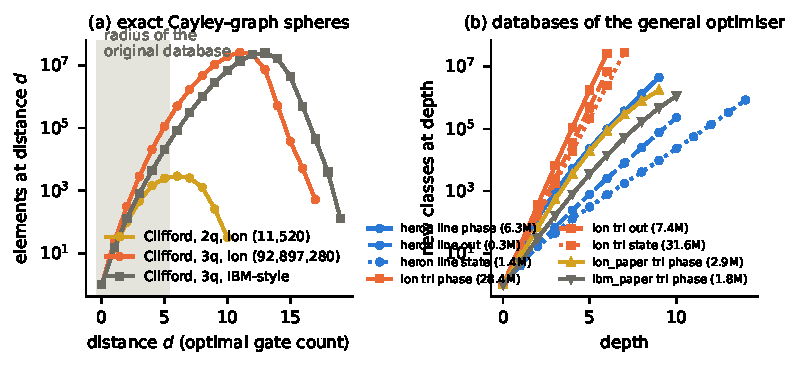
\includegraphics[width=\textwidth]{figs/fig_growth.pdf}
\caption{(a) Sphere sizes of the exact Cayley graphs used as ground truth. The shaded band is the radius of the original
database. The Clifford+T sphere sizes keep growing roughly tenfold per level, since the group is infinite. (b) Level sizes of the
general optimiser's databases (keys per depth, one curve per device, topology and equivalence notion).}\label{fig:growth}
\end{figure}

\begin{figure}[t]
\centering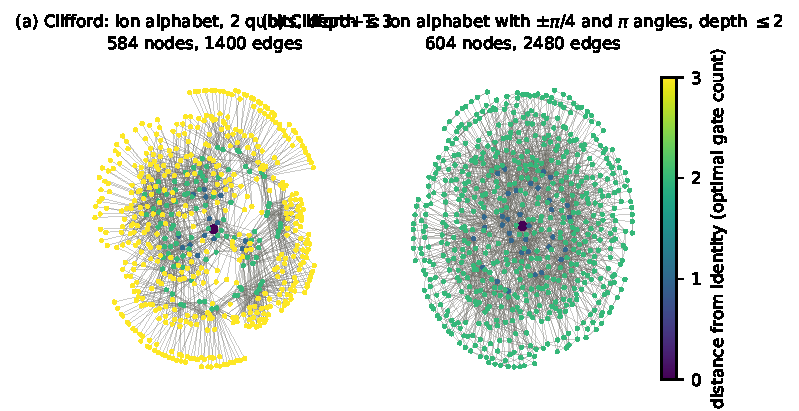
\includegraphics[width=\textwidth]{figs/fig_compute_graph.pdf}
\caption{Compute graphs of comparable size, nodes coloured by exact distance from the identity. (a) Two-qubit Clifford
group, ion alphabet, depth $\le3$. Many short words coincide, and the ball closes up. (b) Two-qubit Clifford+T, depth
$\le2$. Almost every word is new.}\label{fig:cg}
\end{figure}

For $n=3$, the numbers of elements that need exactly $0,1,\dots,6$ entangling gates are 13\,824, 373\,248, 5\,971\,968,
38\,486\,016, 42\,052\,608, 5\,971\,968 and 27\,648 (mean \TwoQThreeMean). By local equivalence of $\RXX(\frac\pi2)$ and $\CZ$
the distribution is the same for both alphabets.

\subsection{Beyond Clifford: exact two-qubit Clifford+T distances}\label{sec:cliffordt}

With angles in $\{\pm\frac\pi4,\pm\frac\pi2,\pi\}$ the ion alphabet ($\RX,\RY,\RZ$ on each qubit and
$\RXX(\pm\frac\pi4,\pm\frac\pi2)$, giving 34 gates on two qubits, the grid of the journal version of~\cite{rosenhahn2025}) is
universal, and the group is infinite. Up to a global phase, however, every generator has entries in the ring
$\Dw=\mathbb Z[1/\sqrt2,\omega]$, $\omega=e^{i\pi/4}$ (e.g.\ $\RZ(\frac\pi4)\propto\mathrm{diag}(1,\omega)$,
$\RX(\theta)\propto H\,\RZ(\theta)\,H$, $\RXX(\theta)\propto(H\otimes H)\,\mathrm{diag}(1,e^{i\theta},e^{i\theta},1)\,(H\otimes
H)$), and so does every circuit~\cite{giles2013}. We represent a unitary exactly as $U=M/\sqrt2^{\,k}$ with $M$ a matrix
over $\Zw$, stored as four integer coefficients per entry in the $\mathbb Z$-basis $1,\omega,\omega^2,\omega^3$.

\begin{lemma}[Exact projective canonical form]\label{lem:canon}
For $U$ with entries in $\Dw$ let $p$ be the first non-zero entry in row-major order and $P(U)_{ij}=U_{ij}\overline{U_p}$.
Then $P(U)$ has entries in $\Dw$, and $V=e^{i\varphi}U$ for some $\varphi$ if and only if $V$ has the same first non-zero
position and $P(V)=P(U)$. Writing $P(U)=M'/\sqrt2^{\,k'}$ with the smallest $k'\ge0$ for which $M'$ has entries in $\Zw$
makes the pair $(M',k')$ unique.
\end{lemma}
\begin{proof}
$\Dw$ is closed under products and conjugation ($\overline\omega=-\omega^3$). If $V=e^{i\varphi}U$, the zero patterns agree
and $V_{ij}\overline{V_p}=U_{ij}\overline{U_p}$. Conversely, $P(V)=P(U)$ at $(i,j)=p$ gives $|V_p|=|U_p|$, so
$V_p=e^{i\varphi}U_p$ for some $\varphi$, and then $V_{ij}=U_{ij}\overline{U_p}/\overline{V_p}=e^{i\varphi}U_{ij}$.
For uniqueness, note that $1,\omega,\omega^2,\omega^3$ is a $\mathbb Z$-basis of $\Zw$ and that the smallest common exponent is unique.
Divisibility by $\sqrt2=\omega-\omega^3$ is decided exactly by checking that all coefficients of $M\sqrt2$ are even.
\end{proof}

We hash the canonical forms into 64-bit keys, grow a breadth-first ball of radius \CTRadius\ (\CTBallSize\ elements with
level sizes \CTBallLevels, built in \CTBallMinutes\ minutes) and certify afterwards that the number of distinct keys equals the
number of distinct canonical forms, so no collision occurred and the ball is exact. The exact distance of any circuit of
length at most $R+R'$ follows by meet in the middle. If $U=XY$ with $|Y|=j\le R'$, then $X=UY^\dagger$ lies in the ball,
and $|U|=\min_j\bigl(j+\min_{Y\in S(j)}|UY^\dagger|\bigr)$. With spheres kept up to $R'=\CTRadius-1$ this certifies
optimal lengths up to \CTCertified, and a certified lower bound beyond.

\paragraph{Planted benchmarks.} Long circuits are mostly beyond any certifiable radius, so we \emph{plant} the optimum.
Starting from a random core $c$ whose exact optimal length equals $|c|$, we repeatedly pick a random window $W$ (up to four
gates) and a random word $r$ (up to three gates), compute a geodesic $s$ of $W r^{-1}$ exactly, and replace $W$ by $r$
followed by $s$. Since $\ev(s)\ev(r)=\ev(W)$, the unitary, and hence the certified optimum $|c|$, is unchanged. Since windows
overlap as the circuit grows, the planted structure is not local. This is the analogue, for gate count, of the known-optimal
benchmarks used for qubit mapping~\cite{tan2021queko}.

%=====================================================================
\section{Experiments}\label{sec:exp}

\paragraph{Verification.} Every output is checked against its input. Exact mode is checked by $\op{(U-V)\psi}$ on random
states (statevector on the active qubits, maximum $\IonMaxExactErr$), state-aware mode by the total-variation distance (TVD) of the
output distributions on $|0^n\rangle$ (maximum $\IonMaxStateErr$), approximate mode against the tracked bound, and
Clifford+T outputs by exact equality in $\Dw$. Every output is also checked to be native and to use only coupled pairs.
All \PaperBenchN\ paper-benchmark outputs, all 720 hardware-suite outputs, and all Clifford+T and layout outputs pass.
BQSKit outputs are checked in the same way, up to global phase and BQSKit's final qubit permutation. Outputs of the
large-circuit suite (Section~\ref{sec:large}) are checked by replay certificates.

\subsection{The original benchmarks against ground truth}

We run the general optimiser with the semantics of~\cite{rosenhahn2025} (up to phase, gate count, $\pm\frac\pi2$
alphabets, all-to-all) on the same settings and seeds, namely Tables~III/IV (3 qubits, 300 gates, 20 circuits each), the journal's
4-qubit statistics (100 circuits) and Table~V (15 qubits, 500 gates, 10 circuits). ``Original'' is our faithful port of the
authors' V2, which reproduces their single-circuit 3-qubit result (\FaithIon\ vs.\ 45 gates).

\begin{table}[t]
\caption{Mean gate counts on the original benchmarks. $^*$Original and Qiskit at 4 qubits use the first 30 circuits.
Qiskit is level 3, orig.\ is the original method, and Cliff.\ CW uses adaptive commutation-aware windows with the exact
Clifford tables (Appendix~\ref{app:cliff}), which the general optimiser does not use. Optimum is the proven optimum or a
certified lower bound, and \#opt.\ counts the circuits on which the general optimiser is optimal. All \PaperBenchOk/\PaperBenchN\ outputs verified and native.}\label{tab:paperbench}
\small
\begin{tabular*}{\textwidth}{@{\extracolsep\fill}lcccccc}
\toprule
setting & Qiskit & orig. & Cliff.\ CW & general & optimum & \#opt.\\
\midrule
T3, ion, 3q & \QThreeIon & \TThreePaper & -- & \TThreeGen & \TThreeOpt & \TThreeAtOpt/20\\
T4, IBM-style, 3q & \QThreeIbm & \TFourPaper & -- & \TFourGen & \TFourOpt & \TFourAtOpt/20\\
journal, ion, 4q & \QFourIon$^*$ & \NjpIonPaper$^*$ & \NjpIonCliff & \NjpIonGen & $\ge$\LBFourIon & --\\
journal, IBM-style, 4q & \QFourIbm$^*$ & \NjpIbmPaper$^*$ & \NjpIbmCliff & \NjpIbmGen & $\ge$\LBFourIbm & --\\
T5, IBM-style, 15q & \TFiveLThree & \TFivePaper & \TFiveCliff & \TFiveGen & -- & --\\
\botrule
\end{tabular*}
\end{table}

\begin{figure}[t]
\centering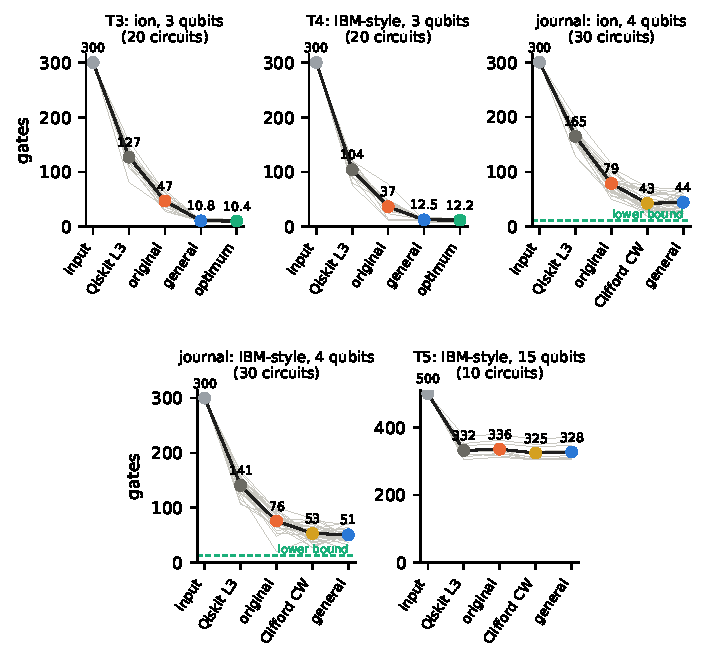
\includegraphics[width=\textwidth]{figs/fig_paper_flow.pdf}
\caption{From the input to the output of every method on the original benchmarks. Grey lines are individual circuits (paired by seed) and
the black line is the mean. The dashed line at 4 qubits is the certified lower bound of Proposition~\ref{prop:count}.}\label{fig:paperflow}
\end{figure}

\begin{figure}[t]
\centering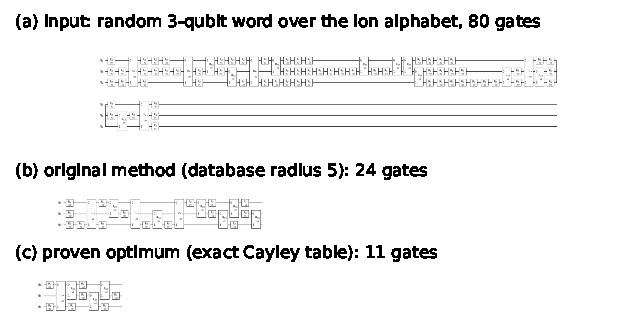
\includegraphics[width=\textwidth]{figs/fig_example_paper.pdf}
\caption{A random 3-qubit word over the ion alphabet (a), the output of the original method (b) and the proven optimum from the
exact Cayley table (c).}\label{fig:expaper}
\end{figure}

Table~\ref{tab:paperbench} and Fig.~\ref{fig:paperflow} show the result. Without knowing that the group is finite or
Clifford, the general optimiser is within 0.4 gates of the proven optimum on average and exactly optimal on 35 of 40
three-qubit circuits, where the original method is $4.5\times$ and $3.0\times$ above the optimum. Fig.~\ref{fig:expaper}
shows a typical case. At four qubits it matches the Clifford-specific optimiser, so knowing the group structure is not what
makes the difference. Large databases and convex windows are. At 15 qubits all methods, Qiskit included, lie within 4\% of one
another, because windows see only a small part of a highly entangled random circuit.

\subsection{Certified Clifford+T benchmarks}

On the two-qubit Clifford+T alphabet we compare the general optimiser (semantics of~\cite{rosenhahn2025}, with an ion database over
exactly this alphabet), the original method (compute graph of depth 4 over the same alphabet) and Qiskit level 3 (which
emits continuous angles, a different alphabet, and is shown for reference) with the certified optimum.

\begin{figure}[t]
\centering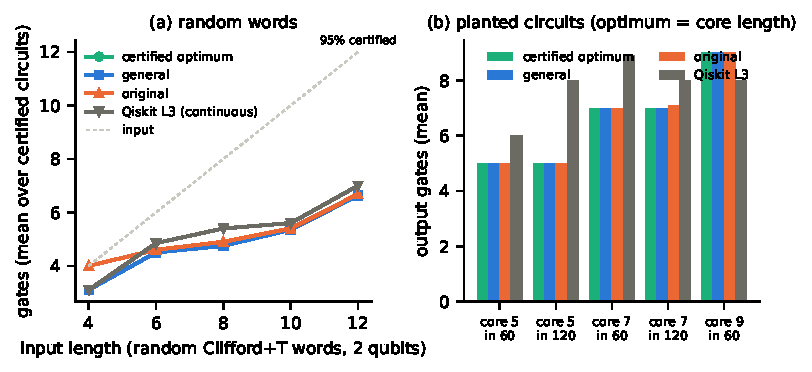
\includegraphics[width=\textwidth]{figs/fig_cliffordt.pdf}
\caption{Clifford+T, two qubits. (a) Random words, mean output length over circuits whose optimum is certified (annotations give
the fraction certified). (b) Planted circuits, a core of the stated length hidden in 60 or 120 gates.}\label{fig:ct}
\end{figure}

\begin{figure}[t]
\centering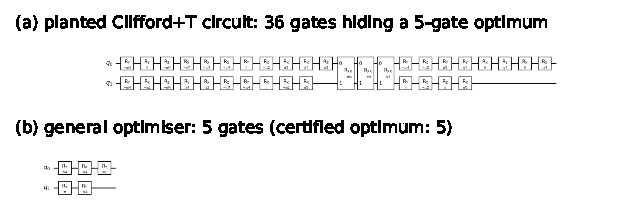
\includegraphics[width=\textwidth]{figs/fig_example_cliffordt.pdf}
\caption{A planted Clifford+T circuit (a) and the output of the general optimiser (b), which equals the certified optimum.}
\label{fig:exct}
\end{figure}

Fig.~\ref{fig:ct} summarises \CTRandN\ random words and \CTPlantN\ planted circuits. On random words with certified optimum
the general optimiser is optimal on \CTRandGenAtOpt\ circuits and the original method on \CTRandOrigAtOpt. On planted
circuits (mean input \CTPlantInputMean\ gates, mean optimum \CTPlantOptMean) the general optimiser reaches the certified
optimum on \CTPlantGenAtOpt/\CTPlantN\ (mean \CTPlantGenMean\ gates), the original method on \CTPlantOrigAtOpt/\CTPlantN\
(mean \CTPlantOrigMean), and Qiskit level 3 returns \CTPlantQiskitMean\ gates on average in its continuous alphabet. All
outputs of the two discrete methods are exactly equal to their inputs in $\Dw$. Fig.~\ref{fig:exct} shows an example.

\subsection{Algorithms on hardware models}

\paragraph{Suite.} We use \HwCircuits\ circuits of 2--\HeronMaxQubits\ qubits and up to \HeronMaxInput\ gates, taken from Nam/VOQC
arithmetic~\cite{nam2018}, QASMBench~\cite{qasmbench} (circuits with classical feed-forward and four that do not parse are
skipped), QFT, QAOA, Heisenberg Trotter steps, EfficientSU2, a Steane encoder and random circuits. Each is compiled by
Qiskit at levels 1 and 3 with the same coupling map and seed. TKET \texttt{FullPeepholeOptimise} runs on the level-1
output followed by a rebase. BQSKit~\cite{bqskit} (version 1.2.1) compiles the same level-1 output at optimisation levels 2
and 3 with its default settings, restricted to the active qubits. On Heron its model is the coupling graph induced on these
qubits, so it may re-place and re-route the circuit within them, and its output is mapped back to the physical qubits so
that ESP uses the same calibration. BQSKit resynthesises blocks of up to three qubits numerically to a tolerance of
$10^{-8}$ per block, so its outputs are approximate.

\begin{table}[t]
\caption{Relative to Qiskit level 3 (\HwCompared\ circuits per device). Count columns are ratios of summed counts, and ESP
is the geometric mean of per-circuit ratios. BQSKit outputs are approximate. The last row applies our optimiser to a
separate BQSKit level-3 run. Nam pf1\_10/pf2\_10 are excluded because Qiskit level 3 drops their $\sim10^{-7}$\,rad rotations
(approximately, not exactly).}\label{tab:hw}
\begin{tabular*}{\textwidth}{@{\extracolsep\fill}lccc c ccc}
\toprule
& \multicolumn{3}{c}{IBM Heron} && \multicolumn{3}{c}{trapped ion}\\\cmidrule{2-4}\cmidrule{6-8}
pipeline & 2q & all & ESP && 2q & all & ESP\\
\midrule
\HwRows
\botrule
\end{tabular*}
\end{table}

\begin{figure}[t]
\centering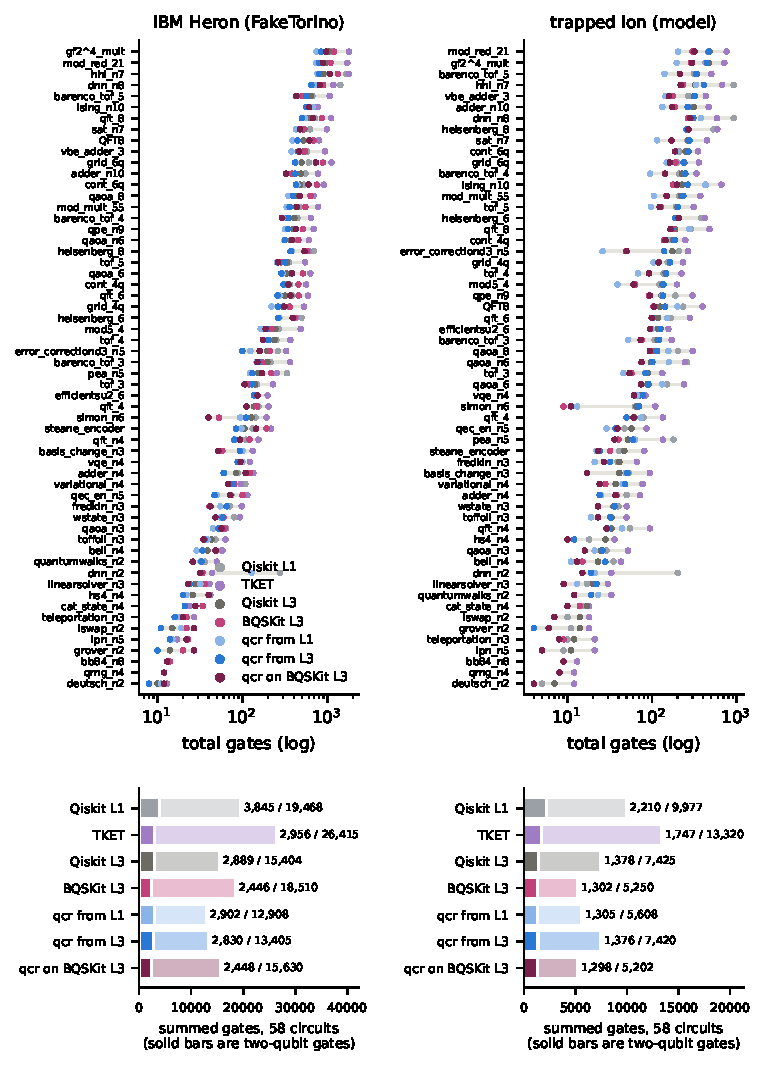
\includegraphics[width=\textwidth]{figs/fig_hw_flow.pdf}
\caption{Hardware suite, from the level-1 compilation to every pipeline's output. The top panel shows total gates per circuit (sorted by
the level-3 count), the bottom panel the sums over all circuits, with two-qubit gates as solid bars.}\label{fig:hwflow}
\end{figure}

\begin{figure}[t]
\centering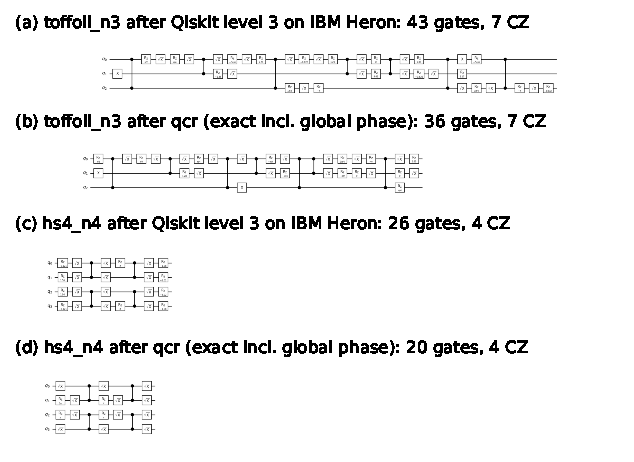
\includegraphics[width=\textwidth]{figs/fig_example_heron.pdf}
\caption{Two QASMBench circuits after Qiskit level 3 on IBM Heron (a, c) and after \qcr\ (b, d). The outputs are equal
including global phase.}\label{fig:exheron}
\end{figure}

Table~\ref{tab:hw} and Fig.~\ref{fig:hwflow} show the results. \emph{Stacked on Qiskit level 3, the optimiser never adds a
two-qubit gate} (\HeronFromLThreeBetter\ circuits better and \HeronFromLThreeEqual\ equal on Heron,
\IonFromLThreeBetter\ better and \IonFromLThreeEqual\ equal on ions) and never lowers ESP. On Heron it removes 13\% of
all gates. $\SX/X$ pulses fall from
\HeronLThreePulse\ to \HeronFromLThreePulse, virtual $\RZ$ from \HeronLThreeRz\ to \HeronFromLThreeRz, and $\CZ$ from
\HeronLThreeTwoq\ to \HeronFromLThreeTwoq\ (Fig.~\ref{fig:exheron}). On ions the total can rise (\IonFromLThreeTotalUp\
circuits) because the calibrated objective trades $\RX/\RY$ pulses for virtual $\RZ$ gates (pulses \IonLThreePulse\ $\to$
\IonFromLThreePulse). The guarantee is on the objective and the two-qubit count, not on the total. Starting from level 1,
the optimiser beats level 3 on Heron in all gates and ESP. Part of the ESP gain ($\times$\HeronEspLOneOverLThree) is due to
Qiskit's level-1 layout already being better than its level-3 layout, our rewriting adding $\times$\HeronEspOursOverLOne.
State/measurement-aware rewriting gives the largest reductions, but \HeronStateEmpty\ (Heron) and \IonStateEmpty\ (ion)
circuits are reversible logic on $|0\cdots0\rangle$ with a fixed output and reduce to the empty circuit, so this mode should
be read per circuit. Median run time is \HeronMedianSec\,s (Heron) and \IonMedianSec\,s (ion) per circuit in single-threaded
Python.

\paragraph{Comparison with resynthesis.} BQSKit is the strongest baseline in the suite (Table~\ref{tab:hw}). Given the same
level-1 input, its level~3 uses fewer two-qubit gates than our exact optimiser on \HeronBqFewerTwoqThanOursLOne\ of
\HwCompared\ Heron circuits and more on \HeronBqMoreTwoqThanOursLOne, and the two reach about the same ESP. Its outputs
contain \HeronBqAllOverOurs\ times as many gates as ours stacked on level 3, because numerical resynthesis leaves many
single-qubit rotations. On ions BQSKit level 3 has fewer gates than every pipeline except our state-aware mode, the same ESP as ours from level 1,
and a higher ESP than ours stacked on level 3 on \IonBqHigherEspThanOursLThree\ of \HwCompared\ circuits. Its outputs differ from the input by a median of $\HeronBqMedErr$
(maximum $\HeronBqMaxErr$ on Heron and $\IonBqMaxErr$ on ions, measured as $\min_\varphi\op{(e^{i\varphi}U-V)\psi}$ on random
states), while ours are exact including global phase. BQSKit level 3 takes \HeronBqMeanSec\,s per Heron circuit on average
with eight worker processes, against \HeronOursMeanSec\,s for our single-threaded optimiser.

\paragraph{Exact rewriting on resynthesised circuits.} The two approaches combine. We ran BQSKit level~3 again on the
level-1 input and applied our exact optimiser (calibrated cost) to its output. BQSKit is not deterministic across runs, so
this input has \HeronStackInTwoq\ two-qubit and \HeronStackInAll\ total gates on Heron, close to but not identical with the
run in Table~\ref{tab:hw}, and each stacked output is compared with its own input. Our optimiser never adds a two-qubit gate
and never lowers ESP. On Heron it removes two-qubit gates on \HeronStackTwoqDown\ of \HwCompared\ circuits
($\times$\HeronStackTwoqOverBq), reduces the total from \HeronStackInAll\ to \HeronStackAll\ gates
($\times$\HeronStackAllOverBq) and raises ESP on \HeronStackEspUp\ circuits ($\times$\HeronStackEspOverBq, geometric mean).
Most of the saving is in the single-qubit rotations that numerical resynthesis leaves behind. On ions BQSKit's output is
already lean, and the gain is small ($\times$\IonStackAllOverBq\ in total gates, ESP higher on \IonStackEspUp\ circuits but
unchanged in the geometric mean). The total count rises on \HeronStackTotalUp\ Heron and \IonStackTotalUp\ ion circuits,
where the calibrated cost trades cheap gates for fewer expensive ones. Each rewrite is exact, and the stacked outputs
differ from BQSKit's by at most $\HeronStackMaxErr$ (floating-point rounding). The extra step takes \HeronStackMeanSec\,s
per Heron circuit and \IonStackMeanSec\,s per ion circuit on average.

\subsection{Large circuits}\label{sec:large}

\paragraph{Suite.} To test scale we ran the same pipelines on \LargeCircuits\ circuits of the Nam/VOQC
suite~\cite{nam2018} with 14 to 100 qubits. They are decomposed to $\{U3, CX\}$ and compiled by Qiskit for the 133-qubit
Heron model and for an all-to-all ion model with one ion per qubit. Our optimiser runs in the calibrated exact mode as before.
The product-formula circuits pf1 and pf2 (\LargeHeronPfN\ per device) are excluded from the comparison for the reason given
for Table~\ref{tab:hw}, as Qiskit level~3 removes almost all of their gates. Circuits with a certificate awaiting
re-check (\LargeHeronPending\ on Heron, \LargeIonPending\ on ions, see below) are excluded as well. This leaves
\LargeHeronN\ Heron circuits of \LargeHeronMinQubits--\LargeHeronMaxQubits\ qubits with up to \LargeHeronMaxInput\ input
gates, and \LargeIonN\ ion circuits with up to \LargeIonMaxInput\ input gates. BQSKit was not run on this suite.

\begin{table}[t]
\caption{Large circuits, relative to Qiskit level 3 (\LargeHeronN\ Heron and \LargeIonN\ ion circuits of up to
\LargeHeronMaxQubits\ qubits). Count columns are ratios of summed counts, and ESP is the geometric mean of per-circuit
ratios. Every output of our optimiser has an accepted replay certificate.}\label{tab:large}
\begin{tabular*}{\textwidth}{@{\extracolsep\fill}lccc c ccc}
\toprule
& \multicolumn{3}{c}{IBM Heron} && \multicolumn{3}{c}{trapped ion}\\\cmidrule{2-4}\cmidrule{6-8}
pipeline & 2q & all & ESP && 2q & all & ESP\\
\midrule
\LargeRows
\botrule
\end{tabular*}
\end{table}

\paragraph{Results.} Table~\ref{tab:large} shows the picture of the 60-circuit suite with larger margins on Heron. Stacked
on Qiskit level~3, the optimiser removes \LargeHeronFromLThreeAllSaved\ of all gates and \LargeHeronFromLThreeTwoqSaved\ of the
two-qubit gates on Heron. It removes two-qubit gates on \LargeHeronFromLThreeBetter\ of \LargeHeronN\ circuits, never adds
one, and raises ESP by $\times$\LargeHeronFromLThreeEsp\ in the geometric mean. On ions it never adds a two-qubit gate and
never lowers ESP. The total never rises on Heron and rises on \LargeIonFromLThreeTotalUp\ ion circuits, again
because the calibrated cost trades pulses for virtual $\RZ$ gates. Starting from level~1, the optimiser ends with fewer gates
than level~3 on all \LargeHeronN\ Heron circuits but with more two-qubit gates on \LargeHeronLOneTwoqMore\ of them, since
level~3 routing and resynthesis find entangling structure that local rewriting does not reach. On ions, where no routing is
needed, it uses fewer two-qubit gates than level~3 on \LargeIonLOneTwoqFewer\ circuits and more on none.

\paragraph{Certificates.} Of the \LargeOutputs\ outputs of our optimiser, \LargeCertOk\ have an accepted replay certificate.
A certificate replays up to \LargeCertMaxSteps\ steps in at most \LargeCertMaxSec\,s (median \LargeCertMedSec\,s), against up
to hours for the optimisation itself, and the summed residuals stay below $\LargeCertMaxErr$. The first version of the
checker rejected \LargeCertFirstRejected\ certificates. It checked the whole phase repair as one block, which exceeds its
limit of 12 wires when the repair touches two distant parts of a wide circuit. The current checker treats each repaired
patch separately. The optimiser is deterministic. Rerunning it on the \LargeCertRechecked\ cases re-checked so far reproduced
their outputs exactly, and the current checker accepted both. The remaining \LargeCertPending\ are excluded from Table~\ref{tab:large} until
their re-check is done.

\paragraph{Run time.} Table~\ref{tab:runtime} lists median run times. Qiskit needs well under a second per circuit and
TKET a few seconds. On the 60-circuit suite our optimiser takes seconds per circuit, like BQSKit level~2 and less than
BQSKit level~3, which used eight worker processes. On the large suite it takes minutes and up to \LargeHeronMaxSec\,h per
circuit, in single-threaded Python with five circuits sharing eight cores. Run time is the main cost of the method at this
scale. Sweeps over non-overlapping windows could run in parallel, which we have not done.

\begin{table}[t]
\caption{Median run time per circuit in seconds. BQSKit was run only on the 60-circuit suite, and Qiskit level~1 was not
timed there. The large suite ran five circuits at a time on eight cores.}\label{tab:runtime}
\begin{tabular*}{\textwidth}{@{\extracolsep\fill}lcc c cc}
\toprule
& \multicolumn{2}{c}{60-circuit suite} && \multicolumn{2}{c}{large suite}\\\cmidrule{2-3}\cmidrule{5-6}
pipeline & Heron & ion && Heron & ion\\
\midrule
\RuntimeRows
\botrule
\end{tabular*}
\end{table}

\subsection{Choosing the objective}

We ran the optimiser with $c_{\rm count}$, $c_{w2}$ and $c_{\rm cal}$ and simulated each output with noise (on Heron
the calibrated gate errors of the actual physical qubits, on ions depolarising noise at the model rates), using the exact TVD between
ideal and noisy output distributions from density matrices on the \HeronTvdCircuits\ circuits with at most eight active
qubits (Table~\ref{tab:tvd}). The calibrated cost is at least as good as the alternatives on both devices and beats Qiskit
level 3 on \HeronCalBeatsLThree/\HeronTvdCircuits\ Heron circuits. The two-qubit-weighted count is a good proxy where no
calibration exists.

\begin{table}[t]
\caption{Mean noisy-simulation TVD by objective (lower is better).}\label{tab:tvd}
\begin{tabular*}{\textwidth}{@{\extracolsep\fill}lccccc}
\toprule
& Qiskit L1 & Qiskit L3 & ours, count & ours, $w2$ & ours, calibrated\\
\midrule
Heron & \HeronTvdLOne & \HeronTvdLThree & \HeronTvdCount & \HeronTvdWTwo & \HeronTvdCal\\
ion & \IonTvdLOne & \IonTvdLThree & \IonTvdCount & \IonTvdWTwo & \IonTvdCal\\
\botrule
\end{tabular*}
\end{table}

\subsection{Layout-aware rewriting}

On Heron we compare, for the \LayN\ circuits of the suite, Qiskit level 3 without and with the calibrated target
(noise-aware layout), our optimiser on each, relocation after the noise-aware pipeline, and joint layout selection over
four seeds $\times$ two modes. ESP here includes readout errors of the active qubits, and the noisy simulation now includes
readout errors as well.

\begin{figure}[t]
\centering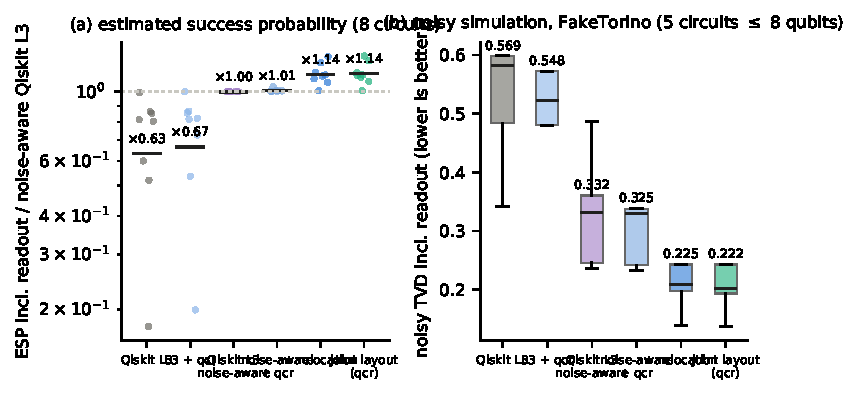
\includegraphics[width=\textwidth]{figs/fig_layout.pdf}
\caption{Layout-aware rewriting on IBM Heron (FakeTorino). (a) ESP including readout relative to Qiskit's noise-aware level 3
(dots are circuits, bars and labels are geometric means). (b) Exact noisy TVD including readout for circuits with at most eight
active qubits (labels: means).}\label{fig:layout}
\end{figure}

\begin{table}[t]
\caption{Layout-aware rewriting on IBM Heron. ESP includes readout, and ratios are geometric means relative to Qiskit's
noise-aware level 3. TVD: mean exact noisy TVD including readout (\LayTvdN\ circuits).}\label{tab:layout}
\begin{tabular*}{\textwidth}{@{\extracolsep\fill}lccc}
\toprule
pipeline & ESP ratio & two-qubit gates (sum) & TVD\\
\midrule
Qiskit L3 (coupling map only) & $\times$\LayEspLThree & \LayTwoqLThree & \LayTvdLThree\\
Qiskit L3, noise-aware & $\times$1.00 & \LayTwoqNA & \LayTvdNA\\
noise-aware + \qcr & $\times$\LayEspNAOurs & \LayTwoqNAOurs & \LayTvdNAOurs\\
noise-aware + \qcr\ + relocation & $\times$\LayEspRel & \LayTwoqRel & \LayTvdRel\\
joint layout selection (\qcr) & $\times$\LayEspJoint & \LayTwoqJoint & \LayTvdJoint\\
\botrule
\end{tabular*}
\end{table}

Table~\ref{tab:layout} and Fig.~\ref{fig:layout} show that placement dominates: Qiskit's own noise-aware layout already raises
ESP by a factor of $1/$\LayEspLThree\ over the coupling-map-only layout. Relocation after rewriting adds $\times$\LayEspRel, and
joint selection $\times$\LayEspJoint, with noisy TVD lower than the noise-aware baseline on \LayJointBeatsNA/\LayTvdN\ circuits.
Joint selection chose a noise-aware candidate in \LayJointNAShare\ of the circuits, i.e.\ the best final layout is often not the
one Qiskit ranks best before optimisation.

%=====================================================================
\section{Discussion and limitations}\label{sec:discussion}

\paragraph{What the ground truth shows.} For the discrete alphabets of~\cite{rosenhahn2025}, local rewriting is rewriting on a
Cayley graph, controlled by a few exact quantities (diameter, growth, shortest odd relation, mixing rate), and the original
method leaves most of the possible reduction unrealised because its database radius is below the exactness threshold. A
general optimiser with large hashed databases and convex windows closes almost all of the gap without exploiting the group
structure, also on certified Clifford+T circuits.

\paragraph{Exact rewriting and resynthesis.} The BQSKit comparison separates two kinds of optimisation. Resynthesis finds
cheaper entangling structure inside blocks that no stored rewrite reaches, and is therefore better at reducing two-qubit
gates. Exact local rewriting is faster, keeps the unitary including global phase, and removes more single-qubit gates.
The two are complementary rather than competing. Applied after resynthesis, exact rewriting keeps BQSKit's
two-qubit savings and removes a further \HeronStackAllSaved\ of the gates on Heron at no cost in accuracy. A practical
pipeline would use resynthesis for the entangling structure and exact rewriting to clean up.

\paragraph{Limitations.}
(i) \emph{Noise models, not hardware.} ESP and TVD come from calibration snapshots. The simulations contain gate,
relaxation and readout errors but no idle errors or crosstalk, and no real-hardware runs were performed.
(ii) \emph{Global phase.} Our outputs are exact including phase, which costs \HeronPhaseGadgetGates\ single-qubit gates
over the Heron suite. With phase as metadata, as Qiskit, TKET and BQSKit store it, the all-gate ratio from level 1 improves from
$\times0.838$ to $\times0.825$.
(iii) \emph{Baselines.} Quartz and QUESO were not run. Qiskit, TKET and BQSKit use their default settings, and BQSKit
level~4 was run only on the four-qubit benchmark (Table~\ref{tab:four}). BQSKit was not run on the large suite.
(iv) \emph{Scale.} Windows have at most three qubits, the code is single-threaded Python, and feed-forward circuits are out
of scope. Circuits of up to \LargeHeronMaxQubits\ qubits and \LargeIonMaxInput\ gates were tested, where one run takes up to a few
hours. The \LargeCertPending\ outputs whose certificates await re-check, and the largest circuits of the Nam suite, are not yet
reported.
(v) \emph{Clifford+T ground truth} is certified for two qubits and lengths up to \CTCertified, and three-qubit Clifford+T balls
grow too fast for the present implementation.
(vi) \emph{Verification} is numerical (random input states) for the 60-circuit hardware suite and by replay certificates for
the large suite. A certificate proves equality up to the rounding of its local checks. Exact arithmetic is used only for
Clifford and Clifford+T circuits.

\paragraph{Future work.} Two questions remain open. The first is a theory of the self-consistent window $w^\star$, relating
the cascade to Dehn presentations and local geodesics in groups~\cite{gromov1987,epstein1992} and to complete rewriting
systems~\cite{knuthbendix1970}. The second is how to reach the entangling structure that resynthesis finds without giving up
exactness, through larger windows with four-qubit databases and symmetry reduction, or through resynthesised blocks whose
angles are snapped to exactly realisable values and then verified. Error-barred runs on real hardware are the natural next experimental step.

%=====================================================================
\section{Conclusion}\label{sec:conclusion}

Local rewriting becomes reliable when ``equivalent'' is made precise. Each notion is a group action, the database stores its
orbits, and soundness and error accumulation follow. A general optimiser built this way, without using the structure of any
gate set, reaches proven optima on the original three-qubit benchmarks and on planted Clifford+T circuits, improves Qiskit's
level-3 output on real algorithms for Heron and ion models without adding two-qubit gates, and, combined with layout-aware
rewriting, raises the estimated success probability beyond Qiskit's noise-aware layout. Applied after numerical resynthesis
(BQSKit), it keeps the resynthesised two-qubit structure and removes a further \HeronStackAllSaved\ of the gates on
Heron. Exact ground truth, Clifford and
beyond, is what makes such claims checkable.

\backmatter

\bmhead{Acknowledgements}
We thank the authors of~\cite{rosenhahn2025} for publishing their demonstration code, and the developers of Qiskit, Qiskit Aer,
TKET, QASMBench and the VOQC benchmarks.

\section*{Declarations}

\begin{itemize}
\item \textbf{Funding:} No funding was received for this work.
\item \textbf{Competing interests:} The author declares no competing interests.
\item \textbf{Ethics approval and consent to participate:} Not applicable.
\item \textbf{Consent for publication:} Not applicable.
\item \textbf{Data availability:} All raw results, logs and figure data are included in the repository below
  (\texttt{results/}, \texttt{figures/}).
\item \textbf{Materials availability:} Not applicable.
\item \textbf{Code availability:} The implementation (\qcr, Apache License 2.0), every experiment script and the scripts that
  generate all tables, figures and numbers in this paper are available at \url{https://github.com/arnavk23/qcr}.
\item \textbf{Author contribution:} A.K.\ conceived the study, developed the software, performed the experiments and wrote
  the manuscript.
\end{itemize}

\begin{appendices}

\section{Reproduction of the reference method}\label{app:repro}

We ported the authors' MATLAB demonstration code line by line to Python and re-ran every table and figure
of~\cite{rosenhahn2025}. Table~\ref{tab:repro} summarises the outcome (details in the reproduction report in the repository).

\begin{table}[h]
\caption{Reproduction of~\cite{rosenhahn2025}.}\label{tab:repro}
\begin{tabular*}{\textwidth}{@{\extracolsep\fill}p{0.32\textwidth}p{0.14\textwidth}p{0.46\textwidth}}
\toprule
claim & status & detail\\
\midrule
Table I (compute graphs) & exact & identical node and edge counts\\
Figs.~1, 4, 5 (examples) & reproduced & Fig.~4 requires a different gate pool (Theorem~\ref{thm:parity})\\
Tables III/IV, journal 4q & qualified & only with the 24-operator, depth-5 database, which is not stated\\
Table II (V1 $>$ V2 $>$ V3) & qualified & V3 wins only with a tuned forest threshold (recall 30\% at the default)\\
Table V (15 qubits) & not reproduced & ties a current Qiskit (335.9 vs.\ 332.1 gates)\\
Fig.~9 (hardware) & qualified & present at Qiskit levels 0/1, absent at level 3\\
\botrule
\end{tabular*}
\end{table}

\section{Clifford-specific optimisers}\label{app:cliff}

For the alphabets of~\cite{rosenhahn2025}, the exact tables give an \emph{exact-window} optimiser EW-$w$ (all windows of length
at most $w$ on at most three wires replaced by optimal words) and its DAG-convex version CW-$w$. CW-sem grows windows
adaptively while gates commute into them.

\begin{table}[h]
\caption{Mean gate counts in the setting of Tables III/IV of~\cite{rosenhahn2025} (3 qubits, 300 gates, 20 circuits).}\label{tab:gap}
\begin{tabular*}{\textwidth}{@{\extracolsep\fill}lcccccc}
\toprule
& optimum & original & EW-8 & EW-16 & Qiskit L3 & paper (1 circuit)\\
\midrule
ion & \OptIon & \FaithIon & \EWeightIon & \EWsixteenIon & \QThreeIon & 45\\
IBM-style & \OptIbm & \FaithIbm & \EWeightIbm & \EWsixteenIbm & \QThreeIbm & 72\\
time per circuit (ion) & -- & \FaithIonSec\,s & \EWeightIonSec\,s & \EWsixteenIonSec\,s & $<$0.1\,s & --\\
\botrule
\end{tabular*}
\end{table}

\begin{figure}[h]
\centering
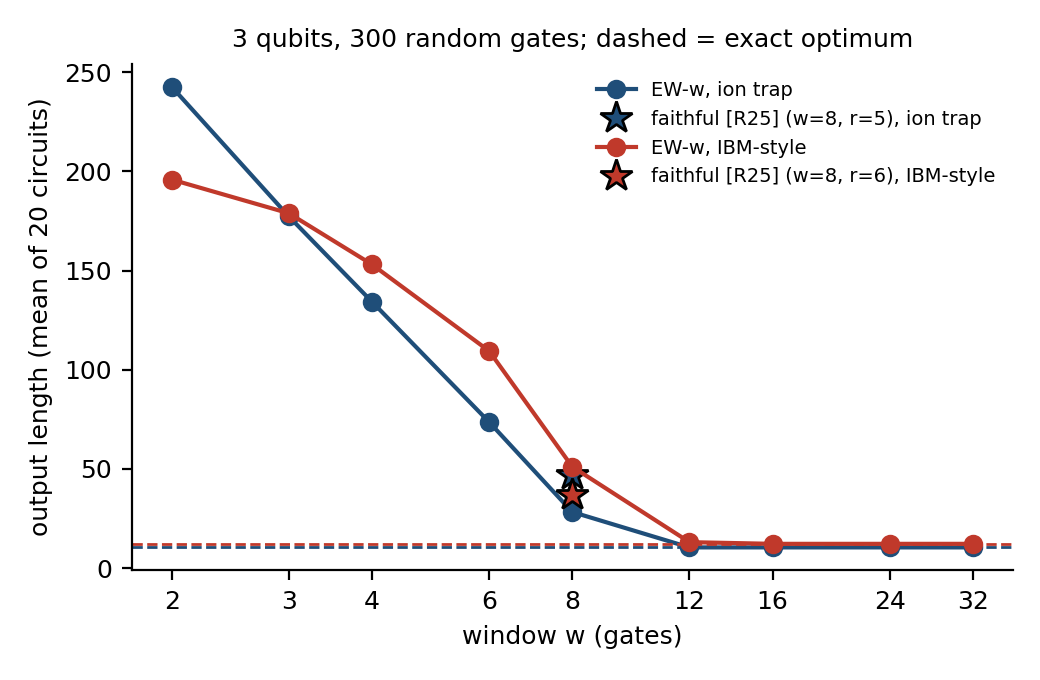
\includegraphics[width=0.49\textwidth]{figs/ext_window.png}\hfill
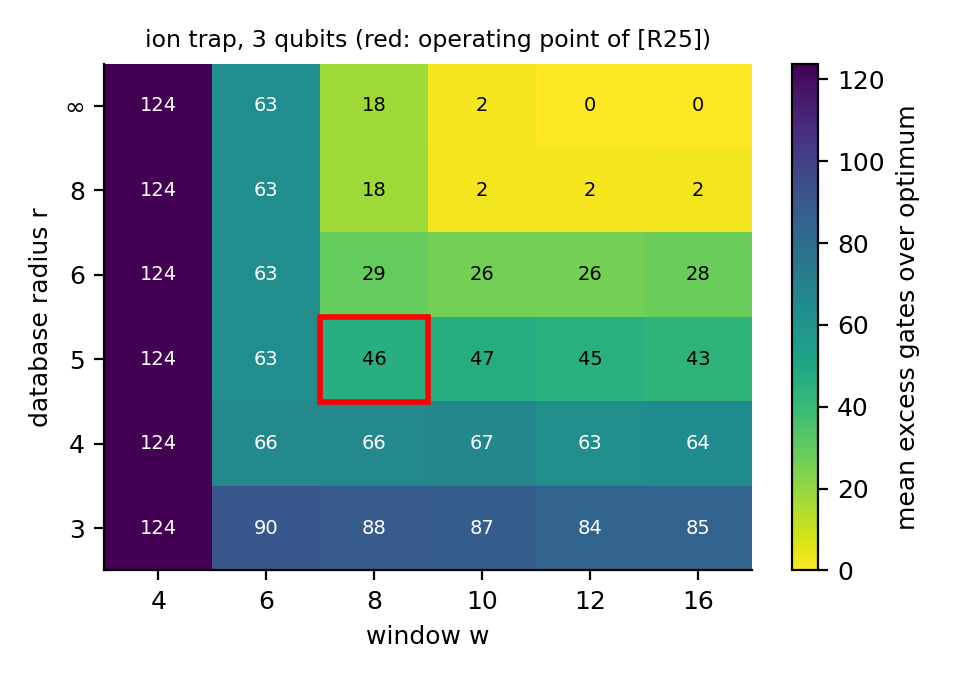
\includegraphics[width=0.49\textwidth]{figs/ext_grid.png}
\caption{Left, the fixed-point length of EW-$w$ against $w$, with the cascade transition near $w^\star$. Right, the mean excess
over the optimum by window $w$ and database radius $r$ (ion), with the original operating point $(8,5)$ marked.}\label{fig:window}\label{fig:grid}
\end{figure}

\GapFindings

\begin{table}[h]
\caption{Journal benchmark (4 qubits, 300 gates, 100 circuits). Original (orig.) and Qiskit level 3 use the first 30 circuits. Published (publ.)
numbers are from the journal version of~\cite{rosenhahn2025}. BQSKit level 4 is our run on the first \BqFourN\ circuits, with the
same gate set at continuous angles (approximate, all-to-all).}\label{tab:four}
\small\setlength{\tabcolsep}{3pt}
\begin{tabular*}{\textwidth}{@{\extracolsep\fill}lcccccccc}
\toprule
& bound & CW-sem & CW-24 & EW-16 & orig. & publ. & Qiskit & BQSKit\\
\midrule
ion, total & $\ge$\LBFourIon & \NjpIonCliff & \CWFourIon & \EWFourIon & \FaithFourIon & 111 & \QFourIon & \BqFourIon\\
ion, $\RXX$ & -- & -- & \CWFourIonTwoQ & \EWFourIonTwoQ & \FaithFourIonTwoQ & 43 & \QFourIonTwoQ & \BqFourIonTwoQ\\
IBM-style, total & $\ge$\LBFourIbm & \NjpIbmCliff & \CWFourIbm & \EWFourIbm & \FaithFourIbm & 107 & \QFourIbm & \BqFourIbm\\
IBM-style, $\CZ$ & -- & -- & \CWFourIbmTwoQ & \EWFourIbmTwoQ & \FaithFourIbmTwoQ & 43 & \QFourIbmTwoQ & \BqFourIbmTwoQ\\
\botrule
\end{tabular*}
\end{table}

\FourFindings

\section{Assessment of the reference method}\label{app:assess}

For completeness we list the issues found while reproducing~\cite{rosenhahn2025}, to make the comparison
transparent.
(1) \emph{Structure.} The gate sets are Clifford, but floating-point comparisons with three different tolerances
($10^{-5}$, $10^{-4}$, $10^{-3}$) and a linear database scan are used where exact constant-time keys exist.
(2) \emph{Optimality.} Results are compared only with Qiskit.
(3) \emph{Equivalence.} Replacements are up to global phase, which is unsound under control, and no error is tracked.
(4) \emph{Hardware model.} Discrete angles, all-to-all connectivity and total gate count do not match IBM or ion hardware.
(5) \emph{Evaluation.} Random benchmarks mix (Theorem~\ref{thm:mix}), Tables III--V use one circuit each, and timings compare
interpreted MATLAB with compiled transpilers.
(6) \emph{Search.} Windows are contiguous and commutation is explored by random swaps without a convergence criterion.
(7) \emph{V3.} Forest features and threshold are not reported.
(8) \emph{Hardware evidence.} There is one two-qubit circuit, one run per chip and no error bars.
(9) \emph{Reproducibility.} Only V2 is released, the loop bounds of \texttt{simplereduce} skip the last pair, the database
omits the identity, and the database used for Tables III--V is not stated.

\end{appendices}

\bibliography{refs}

\end{document}
